 \documentclass[11pt, onesided]{book}

%%%%%%%%%%%%%%Include Packages%%%%%%%%%%%%%%%%%%%%%%%%%%
\usepackage{xcolor}
\usepackage{mathtools}
\usepackage[a4paper, total={6in, 8in}, margin=1.25in]{geometry}
\usepackage{amsmath}
\usepackage{amssymb}
\usepackage{paralist}
\usepackage{rsfso}
\usepackage{amsthm}
\usepackage{wasysym}
\usepackage[inline]{enumitem}   
\usepackage{hyperref}
\usepackage{tocloft}
\usepackage{wrapfig}
\usepackage{titlesec}
\usepackage{colortbl}
\usepackage{stackengine} 
%%%%%%%%%%%%%%%%%%%%%%%%%%%%%%%%%%%%%%%%%%%%%%%%%%%%%%%%


%%%%%%%%%%%%%%%Chapter Setting%%%%%%%%%%%%%%%%%%%%%%%%%%
\definecolor{gray75}{gray}{0.75}
\newcommand{\hsp}{\hspace{20pt}}
\titleformat{\chapter}[hang]{\Huge\bfseries}{\thechapter\hsp\textcolor{gray75}{$\mid$}\hsp}{0pt}{\Huge\bfseries}
%%%%%%%%%%%%%%%%%%%%%%%%%%%%%%%%%%%%%%%%%%%%%%%%%%%%%%%%

%%%%%%%%%%%%%%%%%Theorem environments%%%%%%%%%%%%%%%%%%%
\newtheoremstyle{break}
  {\topsep}{\topsep}%
  {\itshape}{}%
  {\bfseries}{}%
  {\newline}{}%
\theoremstyle{break}
\theoremstyle{break}
\newtheorem{axiom}{Axiom}
\newtheorem{thm}{Theorem}[section]
\renewcommand{\thethm}{\arabic{section}.\arabic{thm}}
\newtheorem{lem}{Lemma}[thm]
\newtheorem{cor}{Corollary}[thm]
\newtheorem{defn}{Definition}[thm]
\newenvironment{indEnv}[1][Proof]
  {\proof[#1]\leftskip=1cm\rightskip=1cm}
  {\endproof}
%%%%%%%%%%%%%%%%%%%%%%%%%%%%%%%%%%%%%%%%%%%%%%%%%%%%%%


%%%%%%%%%%%%%%%%%%%%%%%Integral%%%%%%%%%%%%%%%%%%%%%%%
\def\upint{\mathchoice%
    {\mkern13mu\overline{\vphantom{\intop}\mkern7mu}\mkern-20mu}%
    {\mkern7mu\overline{\vphantom{\intop}\mkern7mu}\mkern-14mu}%
    {\mkern7mu\overline{\vphantom{\intop}\mkern7mu}\mkern-14mu}%
    {\mkern7mu\overline{\vphantom{\intop}\mkern7mu}\mkern-14mu}%
  \int}
\def\lowint{\mkern3mu\underline{\vphantom{\intop}\mkern7mu}\mkern-10mu\int}
%%%%%%%%%%%%%%%%%%%%%%%%%%%%%%%%%%%%%%%%%%%%%%%%%%%%%%



\newcommand{\R}{\mathbb{R}}
\newcommand{\N}{\mathbb{N}}
\newcommand{\Z}{\mathbb{Z}}
\newcommand{\Q}{\mathbb{Q}}
\newcommand{\C}{\mathbb{C}}
\newcommand{\T}{\mathcal{T}}
\newcommand{\M}{\mathcal{M}}
\newcommand{\Symm}{\text{Symm}}
\newcommand{\Alt}{\text{Alt}}
\newcommand{\Int}{\text{Int}}
\newcommand{\Bd}{\text{Bd}}
\newcommand{\Power}{\mathcal{P}}
\newcommand{\ee}[1]{\cdot 10^{#1}}
\newcommand{\spa}{\text{span}}
\newcommand{\sgn}{\text{sgn}}
\newcommand{\degr}{\text{deg}}
\newcommand{\pd}{\partial}
\newcommand{\that}[1]{\widetilde{#1}}
\newcommand{\lr}[1]{\left(#1\right)}
\newcommand{\vmat}[1]{\begin{vmatrix} #1 \end{vmatrix}}
\newcommand{\bmat}[1]{\begin{bmatrix} #1 \end{bmatrix}}
\newcommand{\pmat}[1]{\begin{pmatrix} #1 \end{pmatrix}}
\newcommand{\rref}{\xrightarrow{\text{row\ reduce}}}
\newcommand{\txtarrow}[1]{\xrightarrow{\text{#1}}}
\newcommand\oast{\stackMath\mathbin{\stackinset{c}{0ex}{c}{0ex}{\ast}{\Circle}}}
\newcommand{\txt}{Wald's \textit{General Relativity}}

\newcommand{\note}{\color{red}Note: \color{black}}
\newcommand{\remark}{\color{blue}Remark: \color{black}}
\newcommand{\example}{\color{green}Example: \color{black}}
\newcommand{\exercise}{\color{green}Exercise: \color{black}}

%%%%%%%%%%%%%%%%%%%%%%Roman Number%%%%%%%%%%%%%%%%%%%%%%%
\makeatletter
\newcommand*{\rom}[1]{\expandafter\@slowromancap\romannumeral #1@}
\makeatother
%%%%%%%%%%%%%%%%%%%%%%%%%%%%%%%%%%%%%%%%%%%%%%%%%%%%%%%%%

%%%%%%%%%%%%%table of contents%%%%%%%%%%%%%%%%%%%%%%%%%%%%
%\setlength{\cftchapindent}{0em}
%\cftsetindents{section}{2em}{3em}
%
%\renewcommand\cfttoctitlefont{\hfill\huge\bfseries}
%\renewcommand\cftaftertoctitle{\hfill\mbox{}}
%
%\setcounter{tocdepth}{2}
%%%%%%%%%%%%%%%%%%%%%%%%%%%%%%%%%%%%%%%%%%%%%%%%%%%%%%%%%%


%%%%%%%%%%%%%%%%%%%%%Footnotes%%%%%%%%%%%%%%%%%%%%%%%%%%%
\newcommand\blfootnote[1]{%
  \begingroup
  \renewcommand\thefootnote{}\footnote{#1}%
  \addtocounter{footnote}{-1}%
  \endgroup
}
%%%%%%%%%%%%%%%%%%%%%%%%%%%%%%%%%%%%%%%%%%%%%%%%%%%%%%%%%

%%%%%%%%%%%%%%%%%%%%%Section%%%%%%%%%%%%%%%%%%%%%%%%%%%%%
\makeatletter
\def\@seccntformat#1{%
  \expandafter\ifx\csname c@#1\endcsname\c@section\else
  \csname the#1\endcsname\quad
  \fi}
\makeatother
%%%%%%%%%%%%%%%%%%%%%%%%%%%%%%%%%%%%%%%%%%%%%%%%%%%%%%%%%

%%%%%%%%%%%%%%%%%%%%%%%%%%%%%%%%%%%Enumerate%%%%%%%%%%%%%%
\makeatletter
% This command ignores the optional argument 
% for itemize and enumerate lists
\newcommand{\inlineitem}[1][]{%
\ifnum\enit@type=\tw@
    {\descriptionlabel{#1}}
  \hspace{\labelsep}%
\else
  \ifnum\enit@type=\z@
       \refstepcounter{\@listctr}\fi
    \quad\@itemlabel\hspace{\labelsep}%
\fi}
\makeatother
\parindent=0pt
%%%%%%%%%%%%%%%%%%%%%%%%%%%%%%%%%%%%%%%%%%%%%%%%%%%%%%%%%%



\begin{document}

	\begin{titlepage}
		\begin{center}
			\vspace*{0.5cm}
			\Huge \color{red}
				\textbf{Class Notes}\\
			\vspace{0.5cm}			
			\Large \color{black}
			Math 525 - Probability Theory\\
			Professor Dan Burns
			\vspace{1.5cm}

			
\includegraphics[scale=1.15]{hmm.pdf}
			
			
			\vspace{2cm}
			\LARGE
				\textbf{Jinyan Miao}\\
				\hfill\break
				\LARGE Fall 2023\\
			\vspace{1cm}

		\vspace*{\fill}
		\end{center}			
	\end{titlepage}



\tableofcontents
\hfill\break
\hfill\break
\hfill\break
 

\newpage
\chapter{Probability}
\quad There are two basic notions in probability, (1) empirical or sample probability, and (2) models. For (1), one conducts experiments many times and probability is computed by, for instance, number of heads over number of flips of a fair coin. For experiments, one would get a distribution. While on the other hand, (2) is for calculations, but relies on constructions from statistics obtained from experiments. \\

\section[The Probability Space]{\color{red}The Probability Space \color{black}}
\begin{defn}
For given an experiment, a set $\Omega$ can be used to denote the sample space, which is the collection of all possible outcomes of the experiment. An event $E$ is a subset of $\Omega$. 
\end{defn}

\example For flipping a fair coin, one has sample space $\Omega = \{H, T\}$, where $H$ denotes getting a \textit{head} and $T$ denotes getting a \textit{tail}. \\

\example For a \textit{height experiment}, one can have 
$$\Omega=\{\text{all individuals in the U.S. with their current height}\}\, .$$ One can say an event $E= \{ \text{people with height}\geq 160\,\text{cm}\}\subseteq \Omega$. 

\begin{defn}
Let $\Omega$ be a set, $\mathcal{F}$ is called a $\sigma$-algebra on $\Omega$ provided that it satisfies:
\begin{enumerate}[topsep=3pt,itemsep=-1ex,partopsep=1ex,parsep=1ex]
\item $\emptyset \in \mathcal{F}$
\item If $A_n \in \mathcal{F}$ for all $n \in \N$, then $\bigcup_{n\in \N}A_n \in \mathcal{F}$
\item If $A \in \mathcal{F}$, then $A^c \in \mathcal{F}$
\end{enumerate} 
\end{defn}

\remark Note here from Definition 1.0.2, we have $\emptyset, \Omega \in \mathcal{F}$.


\begin{cor}
Let $\Omega$ be a set, and let $\mathcal{F}$ be a $\sigma$-algebra on $\Omega$. \\
If $A_i \in \mathcal{F}$ for all $i \in \N$, then $\bigcap_{i \in \N}A_i \in \mathcal{F}$. \\
If $A, B \in \mathcal{F}$, then $A \setminus (A\cap B)=A \cap B^c \in \mathcal{F}$. 
\end{cor}

\begin{defn}
Given a sample space $\Omega$, let $\mathcal{F}$ be a $\sigma$-algebra of $\Omega$, a probability function $\mathbb{P}: \mathcal{F} \to [0,1]$ satisfies the conditions
\begin{enumerate}[topsep=3pt,itemsep=-1ex,partopsep=1ex,parsep=1ex]
\item $\mathbb{P}(\emptyset) = 0$ and $\mathbb{P}(\Omega) = 1$,
\item If $A_i \subseteq \Omega$ are pairwise disjoint for $i \in \N$, then $\mathbb{P}(\bigcup_{i=1}^\infty A_i) =\sum_{i=1}^\infty \mathbb{P}(A_i)$.
\end{enumerate}
\end{defn}


\example Now for an experiment one independently flips two fair coins, then denoting getting a head as $H$ and getting a tail as $T$, we have $\Omega = \{(T,T), (H,T), (T,H), (H,H)\}$. As the coins are fair, all outcomes in $\Omega$ are equally likely. That is each outcome in $\Omega$ has probability $1/|\Omega|$. For $E \subseteq \Omega$, one has $\mathbb{P}(E) = |E|/|\Omega|$ where $|\cdot |$ is the cardinality function.\\

\remark Probability can be interpreted as an \textit{area} of some subspace of a space. For instance, if $\mathcal{F}$ is a sigma algebra of $\Omega = [0,1]$, then $\mathcal{F}$ contains all intervals $[a,b] \subseteq [0,1]$. Here one could define a probability function by $\mathbb{P}([a,b]) = b-a$, from which we have $\mathbb{P}(\{a\}) = 0$ for $a \in [0,1]$. Note here we have
\begin{align*}
\mathbb{P}\left( \bigcup_{x \in [0,1/2]}\{x\}\right) = \mathbb{P}([0,1/2]) =\frac{1}{2} \neq \sum_{x \in [0,1/2]}\mathbb{P}(\{x\}) = 0
\end{align*}
holds as the union and sum are not countable.

\begin{defn}
Given a sample space $\Omega$, a $\sigma$-algebra $\mathcal{F}$ on $\Omega$, and a probability function $\mathbb{P}$ defined on $\mathcal{F}$, the triple $(\Omega, \mathcal{F}, \mathbb{P})$ is called a probability space. 
\end{defn}

\note Given a probability space $(\Omega, \mathcal{F}, \mathbb{P})$, if $A, B \in \mathcal{F}$ are disjoint, then it is not hard to see that $\mathbb{P}(A\cup B ) = \mathbb{P}(A) + \mathbb{P}(B)$. While if $A, B \in \mathcal{F}$ have non-empty intersection, then we must write
\begin{align*}
\mathbb{P}(A\cup B) = \mathbb{P}(A) + \mathbb{P}(B) - \mathbb{P}(A\cap B)\,,
\end{align*}
as from the fact that we have
\begin{align*}
A \cup B = (A\setminus (A\cap B))\cup (B\setminus (A\cap B)) \cup (A\cap B)\,.
\end{align*}

\begin{lem}
Given a probability space $(\Omega, \mathcal{F}, \mathbb{P})$, for $A , B \in \mathcal{F}$, we obtain 
\begin{align*}
\mathbb{P}(A \setminus (A\cap B)) = \mathbb{P}(A) - \mathbb{P}(A\cap B)
\,.
\end{align*}
\end{lem}

\section[Conditional Probability]{\color{red} Conditional Probability \color{black}}
Given a probability space $(\Omega, \mathcal{F}, \mathbb{P})$, note intuitively that one gets immediately 
\begin{align*}
\mathbb{P}(A) \cdot \mathbb{P}(B|A) = \mathbb{P}(A\cap B)
\end{align*}
holds for $A,B \in \mathcal{F}$, where $\mathbb{P}(B|A)$ denotes the probability of\textit{ $B$ happening given that $A$ has already happened}.
\begin{defn}
Given a probability space $(\Omega, \mathcal{F}, \mathbb{P})$, the conditional probability $\mathbb{P}(B|A)$, the probability of $B\in \mathcal{F}$ happening given that $\mathcal{A}\in \mathcal{F}$ has already happened, is formally defined as
\begin{align*}
\mathbb{P}(B|A)\coloneqq \frac{\mathbb{P}(B\cap A)}{\mathbb{P}(A)}\,,
\end{align*}
for which we require that $\mathbb{P}(A) \neq 0$. 
\end{defn}
\remark Given a probability space $(\Omega, \mathcal{F}, \mathbb{P})$, if $\mathbb{P}(B) = |B|/|\Omega|$ is satisfied for arbitrary $B \in \mathcal{F}$, one has
\begin{align*}
\mathbb{P}(B|A) = \frac{|A\cap B|/|\Omega|}{|A|/|\Omega|} = \frac{|A\cap B|}{|A|}
\end{align*} 
holds for $A,B \in \mathcal{F}$. 

\section[Independence]{\color{red}Independence \color{black}}
\begin{defn}
Given a probability space $(\Omega, \mathcal{F}, \mathbb{P})$, events $A,B \in \mathcal{F}$ are said to be independent of each other provided that we have $\mathbb{P}(A)\cdot \mathbb{P}(B) = \mathbb{P}(A\cap B)$. 
\end{defn}

\note From Definition 2.0.1 and 2.0.2, we see that $A,B \in \mathcal{F}$ are independent, if and only if $\mathbb{P}(B|A) = \mathbb{P}(B)$, if and only if $\mathbb{P}(A |B) = \mathbb{P}(A)$.\\

\note Given a probability space $(\Omega,\mathcal{F},\mathbb{P})$, for $A ,B \in \mathcal{F}$, if $A \cap B = \emptyset$, then it is not hard to see that $A$ and $B$ are not independent. \\

\example A \textit{fair coin}, formally, is a coin that gives the probability of getting a head as $\mathbb{P}(H) = 1/2$ and the probability of getting a tail as $\mathbb{P}(T) = 1/2$. For two \textit{independent} flips, say flip 1 $F_1$ and flip 2 $F_2$, we have
\begin{align*}
\mathbb{P}(F_1 = H,\, F_2 = T) = \mathbb{P}(F_1 = H) \cdot \mathbb{P}(F_2 = T)\,.
\end{align*}

\example Now suppose one has a two stage experiment, rolling a single die two times. If the rollings are independent, then the probability of each outcome, say rolling $1$ the first time and rolling $5$ the second time, denoted as $(1,5)$, is given by
\begin{align*}
\mathbb{P}((1,5)) = \frac{1}{6}\cdot \frac{1}{6} = \frac{1}{36}\, .
\end{align*}

\example For another experiment, one rolls a die and denotes the result as $x$, then rolls a second die, denotes the result as $y$, and discards that result and roll the second die again if $y>x$. The two rollings here are not independent as $\mathbb{P}((1,5)) = 0 \neq 1/36$. 

\begin{lem}[Calculating by Conditioning] 
Given a probability space $(\Omega, \mathcal{F}, \mathbb{P})$, let $\{E_i\in \mathcal{F}\mid i \in \N\}$ be a collection of events such that $E_i$ are pairwise disjoint and $\bigcup_{i \in \N} E_i = \Omega$. Then the we have 
\begin{align*}
\mathbb{P}(A) = \sum_{i\in \N} \mathbb{P}(A|E_i)\cdot P(E_i)\,.
\end{align*}
\end{lem}
\begin{proof}
Note here we can write
\begin{align*}
\mathbb{P}(A|E_i) = \frac{\mathbb{P}(A\cap E_i)}{\mathbb{P}(E_i)}\,,
\end{align*}
hence we have 
\begin{align*}
\mathbb{P}(A|E_i) \cdot \mathbb{P}(E_i) = \mathbb{P}(A\cap E_i)\,.
\end{align*}
Then computing
\begin{align*}
\sum_{i \in \N} \mathbb{P}(A|E_i) \mathbb{P}(E_i) = \sum_{i \in \N} \mathbb{P}(A\cap E_i) = \mathbb{P}\left( \bigcup_{i\in \N}A\cap E_i\right) = \mathbb{P}\left( A\cap \bigcup_{i \in \N} E_i \right) = \mathbb{P}(A)\,,
\end{align*}
the result then follows. 
\end{proof}

\example Now suppose one has a biased coin that flipping a head has probability $\mathbb{P}(H) = p$ and a tail has probability $\mathbb{P}(T) = 1-p = q$. Now one flips the coin twice independently, and gets, for instance, a tail first then a head, $\mathbb{P}(H|T) = p\cdot q$.\\

 Canonical samples for experiments. (1) Coin flips. Independent flips of identical coins. (2A) Urn samples with replacement. Given an urn with finite number $n$ of balls, there will be $k$ species of balls, and one samples the urn, makes a draw of $1$ ball, puts it back, and makes another draw. (2B) Urn samples, but without replacement, that is drawing one ball, without putting it back, and draw the second ball. Here (1) and (2A) are \textit{independent} experiments, and (2B) is not independent in the two draws. \\
 
 Now we consider further that in case (2B), we have $k = 2$ labeled as $B$ and $R$, and $n = 7$, with $3$ $B$'s and $4$ $R$'s in the urn. Drawing twice without replacement, getting a $B$ in the second draw has the probability
 \begin{align*}
 \mathbb{P}(B_2) = \mathbb{P}(B_2 | R_1) \cdot \mathbb{P}(R_1) + \mathbb{P}(B_2 | B_1) \mathbb{P}(B_1) = \frac{1}{2}\cdot \frac{1}{2}+ \frac{1}{3}\cdot \frac{3}{7}\,.
 \end{align*}
The probability of getting $B$ at the third drawing without replacement, $R$ in the second drawing without replacement, and $R$ in the first drawing, is given by
\begin{align*}
\mathbb{P}(B_3,R_2,R_1) = \mathbb{P}(B_3 | (R_2,R_1))\cdot \mathbb{P}(R_2|R_1) \cdot \mathbb{P}(R_1)\,.
\end{align*}

\example Now consider we have an experiment with a fair coin, flipping independently until we get the first head. Let $A$ denotes the arrival flip of getting the first head. Here we have
\begin{align*}
\mathbb{P}(A = 1) = \frac{1}{2}\,, \qquad \mathbb{P}(A=2) = \frac{1}{4}\,,\qquad \mathbb{P}(A=n) = \frac{1}{2^n}\,.
\end{align*}
Note that, mathematically, 
$$\mathbb{P}(A= \infty) = 1-\left(\sum_{i\in \N} \mathbb{P}(A = i)\right) = 0\,.$$

\example Now suppose that we have an $n$ independent flips of a fair coin. The sample space for such an experiment has a size given by
\begin{align*}
|\Omega| = 2^n
\end{align*}
as we have $2$ outcomes, head or tail, for each flip, and a total of $n$ flips. Now for some $0\leq k \leq n$, one would like to find the probability of getting $k$ heads in $n$ flips. It is not hard to see here
\begin{align*}
\mathbb{P}(\#(H) = k \text{ in }n \text{ flips}) =\binom{n}{k}\left( \frac{1}{2}\right)^k \left( \frac{1}{2}\right)^{n-k} \,.
\end{align*}
Note here we have
\begin{align*}
 \sum_{k=0}^{k\leq n} \binom{n}{k} \left( \frac{1}{2}\right)^k  \left( \frac{1}{2}\right)^{n-k} = 1\,.
\end{align*}
If the coin is instead bias, with probability of getting a head as $p$ and probability of getting a tail as $1 - p = q$. The probability becomes
\begin{align*}
\mathbb{P}(\#(H) = k \text{ in }n \text{ flips}) =\binom{n}{k}p^k q^{n-k} \,.
\end{align*}
One can check that we have
\begin{align*}
\sum_{k=0}^{k\leq n} \binom{n}{k} p^k q^{n-k} = (p+q)^n = 1\,.
\end{align*}
These results of flipping a coin tell us how to compute probability for an urn with two colors, draw made with replacement. \\

\example Now consider that we have an urn that contains balls of two colors, $R$ and $B$, and there are $r$ many $R$'s and $b$ and $B$'s in the urn, with $r+b =n$. One makes $m$ draws without replacement, and one would like to find the probability of obtaining $k$ $R$'s and $m-k$ $B$'s. The number of outcomes here, for a total of $m$ draws from an urn with $n$ balls, is $\binom{n}{m}$, and thus we can write
\begin{align*}
\mathbb{P}(\#(R) = k,\ \#(B) = m-k \text{ in $m$ draws}) = \frac{\binom{r}{k}\binom{b}{n-k}}{\binom{n}{m}}\,.
\end{align*}

\example Now suppose we have a compound experiment. There are three coins, coin $1$, denoted as $c_1$, is fair, coin 2 $c_2$ is biased with $p = 2/3$, and coin 3 $c_3$ is biased with $p = 1/3$. The protocol of the experiment is as follows, first (first step) we flip $c_1$, if one gets a head then (second step) flip $c_2$ twice, and if one gets a tail when flipping $c_1$ (first step), then (second step) flip $c_3$ twice instead. Let $H_1$ denote the event that one gets a head in the first flip in the second step. Let $H_2$ denote the event that one gets a head in the second flip in the second step. Here by conditioning we can write
\begin{align*}
\mathbb{P}(H_1) &= \mathbb{P}(H_1 | c_1 = H) \cdot \mathbb{P}(c_1 = H) + \mathbb{P}(H_1 |c_1 = T) \cdot \mathbb{P}(c_1 = T) \\
&= \frac{2}{3}\cdot \frac{1}{2} + \frac{1}{3}\cdot \frac{1}{2} = \frac{1}{2}\,,
\end{align*}
\begin{align*}
\mathbb{P}(H_2) &= \mathbb{P}(H_2 | c_1 = H) \cdot \mathbb{P}(c_1 = H) + \mathbb{P}(H_2 |c_1 = T) \cdot \mathbb{P}(c_1 = T) \\
&= \frac{2}{3}\cdot \frac{1}{2} + \frac{1}{3}\cdot \frac{1}{2} = \frac{1}{2}\,.
\end{align*}
Furthermore, the probability that one gets heads for both flips in the second step is given by
\begin{align*}
\mathbb{P}(H_1 \cap H_2) 
&= \mathbb{P}(H_1 \cap H_2 | c_1 = H) \cdot \mathbb{P}(c_1 = H) + \mathbb{P}(H_1 \cap H_2 | c_1 = T) \cdot \mathbb{P}(c_1 =T) \\
&= \left( \frac{2}{3}\right)^2 \cdot \frac{1}{2} + \left( \frac{1}{3}\right)^2 \frac{1}{2} = \frac{5}{18}\,.
\end{align*}
However, notice that we have $\mathbb{P}(H_1) \cdot \mathbb{P}(H_2) = 1/4$, from which we see that $\mathbb{P}(H_1 \cap H_2) > \mathbb{P}(H_1) \cdot \mathbb{P}(H_2)$, suggesting that $H_1$ and $H_2$ are not independent of each other. From Bayes Theorem, we can write
\begin{align}
\mathbb{P}(A|B) = \frac{\mathbb{P}(B|A)}{\mathbb{P}(B)}\, \mathbb{P}(A) = \frac{\mathbb{P}(B|A)\cdot \mathbb{P}(A)}{\mathbb{P}(B|A) \cdot \mathbb{P}(A) + \mathbb{P}(B|A^c) \cdot \mathbb{P}(A^c)}\,,
\end{align}
where $\mathbb{P}(A)$ is called the prior, $\mathbb{P}(A|B)$ is called the postorior, $\mathbb{P}(B|A)$ is called the likelihood, and $\mathbb{P}(B)$ is called the marginal. From (1.1) we can calculate
\begin{align*}
\mathbb{P}(c_1 = H |H_1 \cap H_2) = \frac{\mathbb{P}(H_1 \cap H_2 | c_1  = H) \cdot \mathbb{P}(c_1 = H)}{\mathbb{P}(H_1 \cap H_2)} = \frac{4}{5} > \mathbb{P}(c_1 = H)\,.
\end{align*}

\subsection{Independence for more than two events}
\begin{defn}
Given a probability space $(\Omega, \mathcal{F}, \mathbb{P})$, let $\{A_i\} \subseteq \mathcal{F}$ be a collection of $n\geq 2$ distinct events. We say that events in $\{A_i\}$ are independent of each other provided that we have
\begin{align*}
\mathbb{P}(A_1 \cap A_2 \cap \cdots \cap A_n) = \mathbb{P}(A_1) \cdot \mathbb{P}(A_2) \cdot \cdots \cdot \mathbb{P}(A_n)\,.
\end{align*}
\end{defn}
\example Now suppose we flip a fair coin three times, independently. Here we denote the $i$-th flip as $F_i$, here consider three events $A_1= \{F_2 = F_3\}$, $A_2 = \{F_1 = F_2\}$, and $A_3 = \{F_1 = F_2\}$. The three events are independent pairwise, but the three events are not independent of each other as any two of them imply the third. 

\chapter{Discrete Random Variables}
\setcounter{section}{3}
\section[Distributions]{\color{red}Distributions\color{black}}
\textit{Random variables are functions in probability.} 
\begin{defn} 
Given a probability space $(\Omega, \mathcal{F}, \mathbb{P})$, a random variable is a function $X: \Omega \to \R$ that satisfies $\{\omega \in \Omega | X(\omega) \leq x\} \in \mathcal{F}$ for each $x \in \R$, and such function $X$ is said to be $\mathcal{F}$-measurable. 
\end{defn}

\example One flips a fair coin, and one can define $X$ to be the number of heads in such a flip.

\begin{defn}
Given a probability space $(\Omega, \mathcal{F}, \mathbb{P})$ and a random variable $X: \Omega\to  \R$, the function $F: \R \to [0,1] \ \ \ x\mapsto \mathbb{P}(X\leq x)$ is called the accumulative distribution function.
\end{defn}

A Bernoulli random variable $X$ defined on $\Omega = \{H,T\}$ is of a form defined by $X(H) = 1$ and $X(T) = 0$. The distribution of $X$ satisfies $F(x) = 0$ for $x<0$, $F(x) = 1-p$ for $0\leq x< 1$ where $p = \mathbb{P}(H)$, and $F(x) = 1$ for $x \geq 1$.\\

\begin{defn}
Given a probability space $(\Omega, \mathcal{F}, \mathbb{P})$. One can define $I_A:\Omega \to \R$ to be a indicator random variable for event $A \in \mathcal{F}$ by
\begin{align*}
I_A(\omega) = \begin{cases}
1 & \omega \in A\\
0 & \omega \in A^c
\end{cases}\, .\\
\end{align*}
\end{defn}

\note From Definition 4.0.4, $\mathbb{P}(I_A=1) = \mathbb{P}(A)$ and $\mathbb{P}(I_A = 0) = \mathbb{P}(A^c)$. \\
\remark All indicator random variables are Bernoulli random variables. \\

\example Now suppose one is given two events $A$ and $B$, here $I_{A} \cdot I_B = I_{A\cap B}$ is the indicator random variable for the event both $A$ and $B$ happen. Note that $I_A + I_B$ is not necessarily an indicator random variable. $I_A + I_B$ is an indicator random variable if $A\cap B = \emptyset$. 

\begin{lem}
Given a probability space $(\Omega, \mathcal{F}, \mathbb{P})$, and given a random variable $X$ with its distribution function $F$, we have (1) $\mathbb{P}(X>x) = 1-F(x)$ for any $x \in \R$, (2) $\mathbb{P}(x<X\leq y) = F(y) - F(x)$ for any $x,y \in \R$ with $x<y$, and (3) $\mathbb{P}(X=x) = F(x) -\lim_{y\to x^-} F(y)$. 
\end{lem}


In general there are several types of random variables, (1) the discrete random variables, and (2) the continuous random variables.\\


\begin{defn}
Given a probability space $(\Omega, \mathcal{F}, \mathbb{P})$, a random variable $X:\Omega \to \mathcal{R}$ is said to be continuous if its distribution function can be expressed as 
\begin{align*}
F(x) = \int_{-\infty}^x f(u) \, du
\end{align*}
for some integrable function $f:\R \to [0,\infty)$ called the probability density function.
\end{defn}

\begin{defn}
Given a probability space $(\Omega, \mathcal{F}, \mathbb{P})$, a random variable $X:\Omega \to \mathcal{R}$ is said to be discrete if it only takes values in some countable subset of $\R$. The discrete random variable $X$ has proability mass function $f:\R \to [0,1]$ given by $f(x) = \mathbb{P}(X = x)$. 
\end{defn}

\note The probability density function for a continuous random variable and the probability mass function for a discrete random variable will be referred as the distribution of the variable, usually denoted as $f_X$, where $X$ is the random variable.\\

\example \textbf{Binomial Distribution}. For an experiment of $n$ independent flips of a head-tail coin with $p = \mathbb{P}(H)$, we have $\Omega = \{H,T\}^n$. The total number $X$ of heads takes values in the set $\{0,1,2,\cdots, n\}$, and thus is a discrete random variable. The probability mass function is given by $$f(k)=\mathbb{P}(X = k) = \binom{n}{k}p^k q^{n-k}\,,$$ 
where $0 \leq k \leq n$. Here the random variable $X$ is said to have the binomial distribution with parameters $n$ and $p$, denoted as Binomial$[n,p]$, or simply Bin$(n,p)$.\\

\example \textbf{Uniform Distribution}. Here we consider a random variable which has a uniform distribution $f(x)$ on interval $[a,b]\subseteq \R$. Here we can write
$$\mathbb{P}(\alpha \leq x\leq \beta) = \int_\alpha^\beta f(x) \, dx\,.$$ 
Note that $f(x) \geq 0$ for all $x \in \R$ and $\int_\R f(x)\, dx = 1$ are required here. Since $f$ is assumed to be uniform, then we can write $f(x) = c$ for all $x \in \R$, where $c = 1/(b-a)$ follows from the normalization of probability. \\

\example \textbf{Exponential distribution}. Given some probability space $(\Omega, \mathcal{F}, \mathbb{P})$ and a random variable $X:\Omega\to [0,\infty)$ that has a probability density function $f_X(x) =c e^{-\lambda x}$, where $\lambda$ characterizes the decay rate, and $c$ is required by normalization
\begin{align*}
c = \left( \int_0^\infty e^{-\lambda x} \, dx\right)^{-1} = \lambda\,.
\end{align*}
Here $X$ is called an exponential random variable, the exponential distribution with parameter $\lambda$ is denoted as $\text{Exponential}[\lambda]$, or simply $\text{Exp}[\lambda]$.\\

\example \textbf{Poisson Distribution} If a discrete random variable takes values in the set $\N \cup \{0\}$ with a mass function
\begin{align*}
f_X(k) = \frac{\lambda^k}{k!}\, e^{-\lambda}\,,
\end{align*}
with $\lambda>0$, then the variable $X$ is said to be the Poisson distribution with parameter $\lambda$, denoted as $\text{Poisson}[\lambda]$.

\section[Multivariate Random Variables]{\color{red} Multivariate Random Variables\color{red}}
\begin{defn}
Let $X_i$ be random variables, $\vec{X} = (X_1,X_2,\cdots, X_n)$ is a random vector, or a multivariate random variable. The joint accumulative distribution function of a random vector $\vec{X}$ on the probability space $(\Omega , \mathcal{F}, \mathbb{P})$ is the function $f_{\vec{X}}:\R^n \to [0,1]$ defined by $F_{\vec{X}}(\vec{x}) = \mathbb{P}(\vec{X} \leq \vec{x})$ for $\vec{x} \in \R^n$. 
\end{defn}
\note As before, the expression $\vec{X}\leq \vec{x}$ is an abbreviation for the event $\{\omega \in \Omega | \vec{X}(\omega) \leq \vec{x}\}$ for a random vector $\vec{X}$ on the probability space $(\Omega, \mathcal{F}, \mathbb{P})$.\\

\begin{lem}
The joint accumulative distribution function $F_{X,Y}$ of the random vector $(X,Y)$ satisfies 
\begin{enumerate}[topsep=3pt,itemsep=-1ex,partopsep=1ex,parsep=1ex]
\item $\lim_{x,y \to -\infty}F_{X,Y}(x,y) =0$, $\lim_{x,y\to \infty}F_{X,Y}(x,y) = 1$; 
\item If $(x_1,y_1) \leq (x_2,y_2)$, then $F_{X,Y}(x_1,y_1) \leq F_{X,Y}(x_2,y_2)$;
\item $F_{X,Y}$ is continuous from above, that is $\lim_{u,v \to 0^+} F_{X,Y}(x+u , y+v) = F_{X,Y}(x,y)$.
\end{enumerate}
\end{lem}

\example One can think of $2$ coins flipped as a bivariate random variable $(X_1,X_2)$, with $X_i(H) = 1$ and $X_i(T) = 0$. Note here the domain of $X_i$ is the result of $i$-th flip. Here $H_2$, interpreted as the number of $H$ in two flips, is then given by $H_2 = X_1 + X_2$. \\

\note If both $X_1$ and $X_2$ are discrete random variables, and the events $\{\omega |X_1(\omega) = x\}$ are independent of the events $\{\omega |X_2(\omega)= y\}$ for all $x,y \in \R$, then we have
\begin{align*}
\mathbb{P}(X_1 = a,\ X_2 =b) = \mathbb{P}(X_1 = a) \cdot \mathbb{P}(X_2 =b)\,.
\end{align*}
For instance, in the example of flipping two coins, the two flips are independent, but the coin do not have to be fair. 

\begin{defn}
The random variables $X$ and $Y$ on the probability space $(\Omega, \mathcal{F}, \mathbb{P})$ are said to be jointly discrete provided that $(X,Y)$ takes values in some countable subset of $\R^2$. The jontly discrete random variables $(X,Y)$ have joint probability mass function $f_{X,Y}:\R^2 \to [0,1]$ defined by $$f_{X,Y}(x,y) = \mathbb{P}(X=x,Y=y)\,.$$ On the other hand, $X$ and $Y$ are said to be jointly continuous provided that their joint distribution can be expressed as
\begin{align*}
F_{X,Y}(x,y) = \int_{u=-\infty}^x \int_{v=-\infty}^y\, f_{X,Y}(u,v) \, du\, dv
\end{align*}
for $x, y\in \R$ and integrable function $f_{X,Y}$ that is called the joint probability density function of the pair $(X,Y)$. 
\end{defn}

For this chapter, we will focus on the case where $X$ and $Y$ are discrete random variables, and they are jointly discrete. \\


Let $X$ and $Y$ have joint mass function $f_{X,Y}$, one can compute the marginal mass functions $f_X$ and $f_Y$ from the knowledge of $f_{X,Y}$,
\begin{align*}
f_X(x) = \mathbb{P}(X=x) = \mathbb{P}\left( \bigcup_y \{ X = x\} \cap \{Y= y\}\right) = \sum_{y}\mathbb{P}(X=x,\, Y=y) = \sum_y f_{X,Y}(x,y)\,.
\end{align*}
One similarly obtains
\begin{align*}
f_Y(y) = \sum_{x}f_{X,Y}(x,y)\,.
\end{align*}

\begin{defn}
Discrete variables $X$ and $Y$ are independent provided that the events $\{X = x\}$ and the events $\{Y= y\}$ are independent for all $x$ and $y$. 
\end{defn}

\begin{lem}
The discrete random variables $X$ and $Y$ are independent if and only if 
\begin{align*}
f_{X,Y}(x,y) = f_X(x) \cdot f_Y(y)\,,
\end{align*}
for all $x,y \in \R$. More generally, $X$ and $Y$ are independent if and only if $f_{X,Y}(x,y)$ can be factorized as the product $g(x)\cdot h(y)$ of a function of $x$ alone and a function of $y$ alone.  
\end{lem}



\begin{thm}[The Law of Averages]
Let $A_1,A_2,\cdots$ be a sequence of independent events having equal probability $\mathbb{P}(A_i) = p$ where $0 < p <1$. Denote $S_n = \sum_{i=1}^n I_{A_i}$, the sum of indicator functions of $A_i$. Here $S_n$ is a random variable which counts the number of occurrences of $A_i$ for $1\leq i \leq n$. We have $n^{-1}S_n$ converges to $p$ as $n\to \infty$, in the sense that, for all $\epsilon>0$, we can write
\begin{align*}
\lim_{n \to \infty}\mathbb{P}(p-\epsilon \leq n^{-1}S_n \leq p+\epsilon) =1\,.
\end{align*} 
\end{thm}



\section[The Expectation Value]{\color{red}The Expectation Value\color{black}}
\example Let $X$ be a random variable that denotes the grade on an exam worth $100$ points, for a class of $m$ students $s_1,s_2,\cdots, s_m$, that is $X(s_i) = g_i$ is the grade for the $s_i$ student. The average grade for this class is given by
\begin{align*}
\frac{g_1 + g_2 + \cdots + g_m}{m}\,,
\end{align*}
or in other words, we can write the average as
\begin{align*}
\sum_{g=0}^{100} \frac{\#(\{s_i \mid X(s_i) = g\}) \cdot g}{m}\,.
\end{align*}
In this case, the expectation value of $X$, or the mean, average, of $X$, is given by
\begin{align*}
\mathbb{E}(X) \coloneqq \sum_{x_i} \mathbb{P}(X = x_i)\cdot x_i\,.
\end{align*}

\begin{defn}
The mean value, or expectation, or expected value of a discrete random variable $X$ with probability mass function $f_X$ is defined by
\begin{align*}
\mathbb{E}(X) = \sum_{x \in \{x\in \R | f_X(x) >0\}} x\cdot f_X(x) \,.
\end{align*}
\end{defn}

\example For the Bernoulli indicator example, $X$ is defined on $\Omega = \{H,T\}$ with $X(H) = 1$ and $X(T) = 0$. The distribution of $X$ satisfies $F(x) = 0$ for $x<0$, $F(x) = 1-p$ for $0\leq x< 1$ where $p = \mathbb{P}(H)$, and $F(x) = 1$ for $x\geq 1$. Here we have 
\begin{align*}
\mathbb{P}(X = 0) = q\,, \qquad \mathbb{P}(X = 1) = p\,.
\end{align*}
Hence we can write
\begin{align*}
\mathbb{E}(X) = \mathbb{P}(X = 0) \cdot 0 + \mathbb{P}(X = 1) \cdot 1 = p\,.
\end{align*}
\example For the indicator random variable $I_A$ of an event $A$, we have 
\begin{align*}
\mathbb{E}(I_A) = \mathbb{P}(I_A=0)\cdot 0 + \mathbb{P}(I_A = 1) \cdot 1 = \mathbb{P}(A)
\end{align*}
\example For the binomial distribution, that is $X \sim $Binomial$[n,p]$, \footnote{If $X$ is discrete and has a mass function $f$ (or density function if $X$ is continuous), we write $X \sim f$.} we can write
\begin{align*}
\mathbb{E}(X) 
&= \sum_{k=0}^n k\binom{n}{k} p^k q^{n-k} \\
&=p \sum_{k>0}^n k \binom{n}{p} p^{k-1} q^{n-k}\\ 
&= pn \sum_{k>0}^n \binom{n-1}{k-1} p^{k-1} q^{n-k}\\
&= pn \sum_{l=0}^{n-1} \binom{n-1}{l} p^l q^{n-1-l} \\
&= pn
\end{align*}

\begin{defn}
Given a random variable $X$, denoting $\bar{X} = \mathbb{E}(X)$, we can define 
\begin{align*}
\text{Var}(X) = \mathbb{E}((X - \bar{X})^2)
\end{align*} to be the variance of $X$. Here $(X - \bar{X})^2$ is a function of $X$ only, so is a random variable. 
\end{defn}
\note The variance of a variable describes the dispersion about the mean $\mathbb{E}(X)$ of the given variable $X$. \\


\example Suppose we have $X \sim $Bernoulli$[p]$, here we have $\mathbb{E}(X) = p$, and thus 
\begin{align*}
\mathbb{E}((X-p)^2) = (0-p)^2 \cdot q + (1-p)^2 \cdot p = p^2 q+q^2 p = pq(p+q) = pq\,.
\end{align*}
Thus the variance of Bernoulli distribution is $pq$.\\


\note We write $X\sim Y$ for random variables $X$ and $Y$, provided that $X$ and $Y$ are identically distributed, denoted as i.d.. If $X$ and $Y$ are independent and and identically distributed, we denote that they are i.i.d..\\

\example For $c = \sum_{n=1}^\infty 1/n^2 < \infty$, and a random variable that has a probability mass function $p_X(n) = 1/(cn^2)$ for $n \in \N$, we can write
\begin{align*}
\mathbb{E}(X) = \frac{1}{c}\, \sum_{n=1}^\infty n \frac{1}{n^2} = \infty\,.
\end{align*}

\begin{lem}
For discrete random variable $X$, we can write
\begin{align*}
\mathbb{E}(f(X)) = \sum_{x_i} f(x_i)\, p_X(x_i)
\end{align*}
where $x_i$ are possible values of $X$, and $p_X$ is the probability mass function of $X$. 
\end{lem}
\begin{proof}
Here we can write
\begin{align*}
p_{f(X)}(y) = \sum_{f(x) =y} p_X(x)\,.
\end{align*}
Thus we have
\begin{align*}
\mathbb{E}(f(X)) = \sum_{y}y p_{f(X)}(y)
\end{align*}
where $y$ is any possible value of $f(x)$ for $x$ being possible values of $X$, thus
\begin{align*}
\mathbb{E}(f(X)) = \sum_y y\sum_{f(x) = y}p_X(x) = \sum_y f(x)\, p_X(x)\,,
\end{align*} 
which finishes the proof. Note here for $X$ with an infinity number of possible values, we will enforce $\mathbb{E}(|X|) < \infty$. 
\end{proof}


\note Let $(a_i)$ be a sequence, a rearrangement of $(a_i)$ is any reordering of the terms in $(a_i)$. If $\sum_{i=1}^\infty |a_i|<\infty$, then any rearrangement has the same summing result. However, if $\sum_{i=1}^\infty a_i$ exists, but is not absolute convergent, that is $\sum_{i=1}^\infty |a_i| = \infty$, then one can rearrange the terms such that 
\begin{align*}
\sum_{j=1}^\infty a_j = c
\end{align*}
for any $c \in \R$. 


\begin{thm}
Let $X$ and $Y$ be discrete random variables, with finite expectations, then $X+Y$ is also a random variable with expectation
\begin{align*}
\mathbb{E}(X+Y) = \mathbb{E}(X) + \mathbb{E}(Y)\,.
\end{align*}
\end{thm}
\begin{proof}
From Lemma 5.0.1, in particular, we can write
\begin{align*}
\mathbb{E}(X+Y) 
&= \sum_{ij} (x_i+y_j)p_{X,Y}(x_i, y_j)\\
&= \sum_{ij}x_i p_{X,Y} (x_i,y_j) + \sum_{ij}y_j p_{X,Y}(x_i,y_j)\\
&= \sum_{i}x_ip_X(x_i) + \sum_{j} y_j p_Y(y_j) \\
&= \mathbb{E}(X) + \mathbb{E}(Y)\,,
\end{align*}
where $p_{X,Y}$ is the joint mass function of $(X,Y)$, $p_X$ and $p_Y$ are the mass function for $X$ and $Y$, respectively. We thus complete the proof.  
\end{proof}
\note The statement of Theorem 6.1 does not require that $X$ and $Y$ to be independent. \\



\begin{thm}
For random variables $X_1$, $X_2$, $\cdots$, $X_n$, we have
\begin{align*}
\mathbb{E}(X_1+X_2 +\cdots +X_n) = \sum_{i=1}^n \mathbb{E}(X_i)
\end{align*}
\end{thm}

\example Consider $X = \sum_{i=1}^n X_i$, with $X_i$ being i.i.d. as Bernoulli$[p]$. Then we have
\begin{align*}
\mathbb{E}(X) = \sum_{i=1}^n\mathbb{E}(X_i) = pn
\end{align*}

\begin{thm}
For random variables $X$ and $Y$, we have
\begin{align*}
\left( \mathbb{E}(XY)\right)^2 \leq \mathbb{E}(X^2) \cdot \mathbb{E}(Y^2)\,,
\end{align*}
with equality holds if and only if $\mathbb{P}(aX = bY) = 1$ for some real $a$ and $b$, at least one of which is zero.
\end{thm}
\begin{proof}
We assume that $\mathbb{E}(X^2)$ and $\mathbb{E}(Y^2)$ are strictly positive. Let $Z = aX - bY$ for some $a,b \in \R$. Then we can write
\begin{align*}
0\leq \mathbb{E}(Z^2) = a^2 \mathbb{E}(X^2) - 2ab \mathbb{E}(XY) + b^2 \mathbb{E}(Y^2)\,,
\end{align*}
where we notice here the RHS is quadratic in $a$ with at most one real root. Thus its discriminant must be non-positive, for $b\neq 0$, we obtain
\begin{align*}
\left(\mathbb{E}(XY)\right)^2 - \mathbb{E}(X^2) \cdot \mathbb{E}(Y^2) \leq 0\,.
\end{align*}
Furthermore, the discriminant is zero if and only if the quadratic has a real root, and that occurs if and only if $\mathbb{E}(Z^2) = 0$, thus obtaining the result. 
\end{proof}

\section[The Covariance]{\color{red} The Covaraince\color{black}}
\begin{defn}
For random variables $X$ and $Y$, we define the covariance between $X$ and $Y$ as
\begin{align*}
\text{Cov}(X,Y) = \mathbb{E}\left((X-\mathbb{E}(X))\cdot  ( Y -\mathbb{E}(Y))\right)\,.
\end{align*}
\end{defn}
\note Immediately here we have, for random variable $X$, 
\begin{align*}
\text{Cov}(X,X) = \text{Var}(X)\,.
\end{align*}
We see here also 
\begin{align*}
\mathbb{E}(\lambda X) = \lambda \mathbb{E}(X)\,,
\end{align*}
and thus
\begin{align*}
\mathbb{E}\left((\lambda X - \mathbb{E}(\lambda X))^2 \right) = \lambda^2 \text{Var}(X)\,.
\end{align*}


\begin{lem}
Let $X$ and $Y$ be independent random variables. Then we can write
\begin{align*}
\mathbb{E}(X\cdot Y) = \mathbb{E}(X)\cdot \mathbb{E}(Y)
\end{align*}
\end{lem}
\begin{proof}
Here we can write
\begin{align*}
\mathbb{E}(X\cdot Y)  
&= \sum_{ij}x_i y_j p_{X,Y}(x_i, y_j) \\
&= \sum_{ij}x_i y_j p_X(x_i)\, p_Y(y_j)= \left(\sum_i x_i p_X(x_i) \right)\cdot \left( \sum_j y_j p_Y(y_j)\right) = \mathbb{E}(X) \cdot \mathbb{E}(Y)\,,
\end{align*}
thus completing the proof. 
\end{proof}

\begin{cor}
Let $X$ and $Y$ be independent random variables, then we have
\begin{align*}
\text{Cov}(X,Y) = 0\,.
\end{align*}
\end{cor}
\begin{proof}
Here we can write
\begin{align*}
\text{Cov}(X,Y) = \mathbb{E}((X-\mathbb{E}(X) ) (Y - \mathbb{E}(Y))) = \mathbb{E}(X- \mathbb{E}(X)) \cdot \mathbb{E}(Y - \mathbb{E}(Y)) = 0
\end{align*}
\end{proof}

\begin{lem}
For random variables $X$ and $Y$, we have
\begin{align*}
\text{Var}(X+Y)  =  \text{Var}(X) + 2\text{Cov}(X,Y) + \text{Var}(Y)
\end{align*}
\end{lem}
\begin{proof}
Here we can write directly
\begin{align*}
\text{Var}(X+Y) 
&= \mathbb{E}\left(\left(X+Y - \mathbb{E+Y}\right)^2 \right) \\
&= \mathbb{E}\left( \left(X+Y - \mathbb{E}(X) - \mathbb{E}(Y) \right)^2 \right)\\
&= \mathbb{E}\left( \left((X-\mathbb{E}(X)) + (Y-\mathbb{E}(Y))\right)^2 \right)\\
&= \text{Var}(X) + 2\text{Cov}(X,Y) + \text{Var}(Y)\,.
\end{align*}
thus completing the proof.
\end{proof}

\begin{lem}
For a random variable $Y$, we have
\begin{align*}
\text{Var}(Y) = \mathbb{E}(Y^2) - \mathbb{E}(Y)^2\,.
\end{align*}
\end{lem}
\begin{proof}
The result follows from the linearity of expectation,
\begin{align*}
\text{Var}(Y) 
&= \mathbb{E}((Y-\mathbb{E}(Y))^2) \\
&= \mathbb{E}(Y^2 - 2Y\mathbb{E}(Y)+ \mathbb{E}(Y)^2) \\
&= \mathbb{E}(Y^2) - 2\mathbb{E}(Y)\mathbb{E}(Y) + \mathbb{E}(Y)^2 \\
&= \mathbb{E}(Y^2) - \mathbb{E}(Y)^2\,.
\end{align*}
Thus we obtain our result.
\end{proof}


\example Consider $X = \sum_{i=1}^n X_i$, with $X_i$ being i.i.d. as Bernoulli$[p]$.
\begin{align*}
\text{Var}(X) = \sum_i \text{Var}(X_i) = np(1-p)\,.
\end{align*}

\example For geometric random variable $X$ which has mass function $p_X(n) = pq^{n-1}$ with $q = 1-p$, we can write
\begin{align*}
\sum_{n=1}^\infty pq^{n-1} = p \sum_{k=0}^\infty q^k = \frac{p}{(1-q)} = 1\,.
\end{align*}
Note further that we have
\begin{align*}
\sum_{n=0}^\infty x^n = \frac{1}{1-x} \,\qquad \text{for }-1<x<1 \tag{*}
\end{align*}
Here we can compute
\begin{align*}
\mathbb{E}(X) = \sum_{n=1}^\infty npq^{n-1} = p\sum_{n=1}^\infty nq^{n-1} =\frac{p}{(1-q)^2} = \frac{1}{p}\,,
\qquad
\text{Var}(X) = \frac{q}{p^2}
\,,
\end{align*}
where one uses the trick of differentiating, once for expectation and twice for variance, equation (*).\\


%\example For Poisson random variable, taking values $n \in \N \cup \{0\}$, limit as $n \to \infty$ with $p_X = c/n$, we have $X_n \sim $Binomial$[n, c/n]$, and
%\begin{align*}
%\mathbb{E}(X_n) = n\cdot \frac{c}{n} = c
%\end{align*}






\section[Correlation]{\color{red} Correlation Coefficient \color{black}}
Let $X$ and $Y$ be random variables. Let $\mu_X= \mathbb{E}(X)$ and $\mu_Y = \mathbb{E}(Y)$. We know further that we have
\begin{align*}
\text{Cov}(X,Y) = \mathbb{E}((X - \mu_X) (Y-\mu_Y))\,.
\end{align*}
If $X$ and $Y$ are independent, then $\text{Cov}(X,Y) = 0$, as it follows from
\begin{align*}
\mathbb{E}((X - \mu_X) (Y-\mu_Y)) = \mathbb{E}(X - \mu_X)\, \mathbb{E}(Y-\mu_Y) = 0
\end{align*}
when $X$ and $Y$ are independent. There are also some dot product properties, for instance, $\text{Cov}(X,Y)$ is bilinear in $X$ and $Y$, that is
\begin{align*}
&\text{Cov}((a_1X+a_2X),Y) = a_1\text{Cov}(X,Y) + a_2 \text{Cov}(X,Y)\,,\\
&\text{Cov}(X,Y)= \text{Cov}(Y,X)\,, \\
&\text{Var}(X) \cdot \text{Var}(Y)= (\text{Cov}(X,Y))^2\,.
\end{align*}
\begin{defn}
The correlation between random variables $X$ and $Y$ is defined by
\begin{align*}
\text{Correlation}(X,Y) = \frac{\text{Cov}(X,Y)}{\sigma_X\, \sigma_Y} = \rho_{X,Y}\,.
\end{align*}
where $\sigma_X$ and $\sigma_Y$ are the standard deviation of $X$ and $Y$, respectively, defined by the square root of their variances, that is $\sigma_X = \sqrt{\text{Var}(X)}$, and $\sigma_Y = \sqrt{\text{Var}(Y)}$.
\end{defn}
From the Cauchy-Schwarz Inequality, or Theorem 6.3, it is obvious that we have
\begin{align*}
-1\leq \rho_{X,Y} \leq 1\,,
\end{align*}
or in other words, $\rho_{X,Y}$ measures the $\cos(\theta)$ for any $\theta$ between $X$ and $Y$ as vectors. \\

\note For random variable $X$ and $Y$, $\rho_{X,Y} = 0$ implies $\text{Cov}(X,Y) = 0$, that is $X$ and $Y$ are uncorrelated, but such does not imply $X$ and $Y$ being independent. 

\begin{lem}
Let $X$ be a discrete random variable, with $\text{Var}(X) = 0$, then $X = \mu_x$ has probability $1$. 
\end{lem}
\begin{proof}
Here we can write
\begin{align*}
0 = \text{Var}(X) = \sum_{x}(x-\mu_x)^2\, p_X(x)\,,
\end{align*}
as $p_X(x)$ and $(x-\mu_x)^2$ are both nonnegative, we require that $x = \mu_x$ for all possible values of $x$, and thus $X = \mu_x$ has probability $1$. 
\end{proof}

\begin{thm}
Let $X$ and $Y$ be random variables. If $\rho_{X,Y} = 1$, then we have
\begin{align*}
\frac{X - \mu_X}{\sigma_X} = \frac{Y-\mu_Y}{\sigma_Y}\,.
\end{align*}
If we have $\rho_{X,Y} = -1$ instead, then we have
\begin{align*}
\frac{X-\mu_X}{\sigma_X} = -\frac{Y-\mu_Y}{\sigma_Y}\,.
\end{align*}
\end{thm}
%\begin{proof}
%Here we can write
%\begin{align*}
%\mathbb{E}\left( \left(\frac{X-\mu_X}{\sigma_X} - \frac{Y-\mu_Y}{\sigma_Y}\right)^2\right) &=
%\frac{\mathbb{E}((X-\mu_X)^2)}{\sigma_X^2} - \frac{2\mathbb{E}()}{•} + \frac{\mathbb{E}((Y-\mu_Y)^2)}{\sigma_Y^2}
%\textbf{ADD}
%\end{align*}
%\end{proof}
%Theorem 8.1 implies that we have
%\begin{align*}
%\mathbb{E}\left( \left(\frac{X-\mu_X}{\sigma_X} - \frac{Y-\mu_Y}{\sigma_Y}\right)^2\right) = \sum_{x,y}\left( \frac{(x-\mu_X)^2}{\sigma_X} + \frac{(y-\mu_Y)^2}{\sigma_Y} \right)\, p_{X,Y}(x,y) = 0
%\end{align*}
%where $p_{X,Y}$ is the density function for the joint distribution. Here we can denote

\newpage
\section[Conditional Expectation]{\color{red} Conditional Expectation \color{black}}
\begin{defn}
Let $X$ and $Y$ be discrete random variables, we can define a conditional probability mass function from the joint mass function $p_{X,Y}(x,y)$,
\begin{align*}
p_{X|Y}(x|y) = \frac{p_{X,Y}(x,y)}{p_Y(y)}\,, \qquad\text{where }p_Y(y) = \sum_{x} p_{X,Y}(x,y)\,.
\end{align*}
\end{defn} 
\example Now we consider $X\sim\text{Geometric}[p]$. \\
One would like to compute $\mathbb{P}(X=k+n | X\geq n)$, we write
\begin{align*}
\mathbb{P}(X=k+n | X\geq n) = \frac{\mathbb{P}(\{X = k+n\}\cap \{X\geq n\})}{\mathbb{P}(\{X\geq n\})} = \frac{pq^{n+k-1}}{\sum_{l=n}^\infty pq^{l-1}} = \frac{pq^{n+k-1}}{q^{n-1}} =p q^{k-1}
\end{align*}
where 
\begin{align*}
\sum_{l=n}^\infty pq^{l-1} = pq^{n-1} \sum_{l=0}^\infty q^l = pq^{n-1} \frac{1}{1-q} = q^{n-1}
\end{align*}

For discrete random variable $X$ and $Y$, consider the conditional expectation $\mathbb{E}(X|Y)$, which is a random variable as it is a function of $Y$. For instance, consider the experiment of having $Y\in \{0,1\}$, with $Y \sim$ Bernoulli$[1/2]$ and $X$ being the count of flipping coins. If $Y = 0$, then we flip coin$_0$ which has probability $p = 2/3$ twice independently. If $Y = 1$, then we flip coin$_1$ which has probability of getting a head $p = 1/3$ twice independently. $X$ is the count of head obtained in the two flips of a coin.  Here we can write
\begin{align*}
\mathbb{E}(X|Y = 0) = 2 \cdot \frac{1}{3} = \frac{2}{3}\,, \qquad
\mathbb{E}(X|Y=1) = 2\cdot \frac{2}{3} = \frac{4}{3}\,.
\end{align*}
Here we can further compute
\begin{align*}
\mathbb{E}(\mathbb{E}(X|Y)) &= \sum_{y}\mathbb{E}(X|Y = y)\cdot p_Y(y) =\mathbb{E}(X) \\
&= \mathbb{E}(X|Y = 0)\cdot p_Y(0) + \mathbb{E}(X|Y = 1)\cdot p_Y(1)  \\
&= \frac{2}{3}\cdot \frac{1}{2} + \frac{4}{3}\cdot \frac{1}{2} = 1\,.
\end{align*}
Thus we see here it is intuitive to view $\mathbb{E}(X|Y)$ as a random variable taking values in the image of $Y$. 

\begin{thm}
Given discrete random variables $X,Y$, we have
\begin{align*}
\mathbb{E}(\mathbb{E}(X|Y)) = \mathbb{E}(X)\,.
\end{align*}
\end{thm}
\begin{proof}
Here we can write 
\begin{align*}
\mathbb{E}(X|Y=y) = \sum_x x\,\frac{p_{X,Y}(x,y)}{p_Y(y)}\,,
\end{align*}
then we have
\begin{align*}
\mathbb{E}(\mathbb{E}(X|Y)) = \sum_y \sum_x x \, \frac{p_{X,Y}(x,y)}{p_Y(y)}\, p_Y(y) = \sum_x\sum_y  x\, p_{X,Y}(x,y) = \sum_x x p_x(x) = \mathbb{E}(X)\,.
\end{align*}
The result follows.
\end{proof}
\begin{thm}
Given discrete random variables $X,Y$, we have
\begin{align*}
\mathbb{E}(\mathbb{E}(Y|X)\cdot g(X)) = \mathbb{E}(Y\cdot g(X))
\end{align*}
for any function $g$ for which both expectations exist. 
\end{thm}

Note that the variance of a binomial distribution
\begin{align*}
\text{Var}\left(\text{Binomial}[n,p]\right)  = npq \,.
\end{align*}

\example Consider an compound experiment. Here $Y \sim$ Uniform$[0,1]$, and $X$ is the count of two independent flip of a single coin which has a probability of getting a head as $p = Y$. Here we can write
\begin{align*}
\mathbb{E}(\mathbb{E}(X|Y)) = \int_0^1 \mathbb{E}(X|Y=p)\, dp = \int_0^1 2p \, dp = 1\,. 
\end{align*}

\section[Random Walk]{\color{red} Random Walk\color{black}}
Here we consider a symmetric random walk on a line. Starting at the origin $x=0$, one flips a fair coin. If one gets a head, then one walks to the right $x+1$, and if one gets a tail instead, then one walks to the left $x-1$. One is interested in his position after $n$ flips. Let $X_n$ denote the position after $n$ flips. Here we see that $X_1 \in \{-1,1\}$, with probability $\mathbb{P}(X_1=-1) = 1/2$ and $\mathbb{P}(X_1 = 1) = 1/2$. Thus here $X_1 = 2Y-1$ where $Y \sim$ Bernoulli$[1/2]$. Let $Y_i$ be i.i.d. $\sim$ Bernoulli$[1/2]$, then $2Y_i - 1$ can denote the $i$-th step in the walk, and thus we can write
\begin{align*}
X_n = \sum_{i=1}^{n}(2Y_i - 1) =\left( 2\sum_{i=1}^n Y_i \right)- n\,.
\end{align*}
Thus we obtain
\begin{align*}
\mathbb{E}(X_n) = 2\cdot \mathbb{E}\left(\sum_{i=1}^n Y_i \right)- n = 2\cdot \frac{n}{2}  - n = n - n = 0\,.
\end{align*}
Note in fact, there is a theorem saying that, with probability $1$, one will be able to visit $|x| \geq \sqrt{n}$ for large enough $n$. This is an example of a random process, in particular a discrete random process, with discrete $X_1$, $X_2$, $X_2$, $\cdots$, $X_n$, $\cdots$ of random variables, and here $n$ is called the discrete time. The random process describes the probabilistic dynamics, that is the evolution of probability in time $n$. In our case of random walk, once the initial point is picked, the sample space consists of ordered sequences of heads and tails of the coin, or translated into ordered sequences of steps. \\


Another way to describe the random walk is by considering $Y_i$ to be i.i.d. $\sim \text{Bernoulli}[p]$, 
$$X_i = 2Y_i - 1 = \begin{cases}
1 & \mathbb{P}=p\\
-1 &\mathbb{P} = 1-p=q
\end{cases}\,,
$$
we then denote
\begin{align*}
S_n = \sum_{j=1}^n X_j = \text{location of the walker on the line after $n$ steps.}
\end{align*}
Assume here $S_0 = a$ being the initial condition, for some $a \in \Z$.
Notice that the random walk is spatially homogeneous as we have
\begin{align*}
\mathbb{P}(S_n=b | S_0 =a) = \mathbb{P}(S_n = (b-a) | S_0 = 0)\,.
\end{align*}
The random walk is also temporally homogeneous, that is we have
\begin{align*}
\mathbb{P}(S_n = b| S_0 =a) = \mathbb{P}(S_{n+k} = b | S_k=a)
\end{align*}
for some $k\in \N \cup\{0\}$. \\


\example Gambler's Ruin problem.\\
Here we have two players $A$ and $B$, a referee who flips a fair coin independently. If the referee gets a head, then $A$ wins $\$1$ from $B$, and if the referee gets a tail, then $B$ wins $\$1$ from $A$. If any one of them wins all money from the other one, then the game ends. The problem, is quite similar to the random walk problem, but with end points at both sides of the $x$-axis, representing the amount of money that the two persons have initially. Note here $ \pm(M+N)$ is called the absorbing barriers, where $M$ is the money that $A$ has initially, and $N$ is the money that $B$ has initially. 
%If $X_n$ denote the amount of money, minus the initial money, that $A$ has after $n$ rounds, then we can write
%\begin{align*}
%X_{n} = (X_{n-1} + 1) \frac{1}{2} + (X_{n-1} - 1) \frac{1}{2}\,,
%\end{align*}
%thus we have
%\begin{align*}
%(X_{n+1} - X_n ) = \frac{1}{2}( X_n - X_{n-1}) + (X_n - X_{n-1}) \frac{1}{2} = (X_n
% - X_{n-1})\,,
%\end{align*}
%from which we obtain a recursive relation. Note also that $X_0 = 0$, and we can write
%\begin{align*}
%\sum_{i=1}^n (X_i - X_{i-1}) = X_n\,.
%\end{align*}
%We can let $P_n$ denote the amount of money that $A$ has at time $n$, and $Q_n = M+N - P_n$ denote the amount of money that $B$ has at time $n$. Then we see here
%\begin{align*}
%P_{n} = \frac{1}{2}P_{n + 1} + \frac{1}{2}P_{n-1}\,,
%\end{align*}
%thus similarly we obtain
%\begin{align*}
%P_{n+1} - P_n = P_n - P_{n-1}\,.
%\end{align*}
%Suppose here we have $P_n = M+N$, then we can write
%\begin{align*}
%P_n = (P_n - P_{n-1}) + (P_{n-1}-P_{n-2})+\cdots + (P_1 - P_0) + M\,.
%\end{align*}
%Rearranging we obtain
%\begin{align*}
%P_n - M = n\Delta
%\end{align*}
%where $\Delta$ denote $P_i - P_{i-1}$, and one can solve for $\Delta$ using boundary conditions. 


\begin{defn}
A general definition for a random process is $\{X_n\}$, a set of random variables. The random process is said to be Markov provided that
\begin{align*}
\mathbb{P}(X_n | X_0,X_1,\cdots, X_{n-1}) = \mathbb{P}(X_n | X_{n-1})\,.
\end{align*}
That is, a random process is said to be Markov provided that the past history is not needed to determine the probability, only the current state. A Markov process is said to be stationary provided that $\mathbb{P}(X_n | X_{n-1})$ is independent of $n$. 
\end{defn}

\example For the random walk example (second approach, using $S_n$ to denote the location of walker on the line after $n$ steps), we have
\begin{align*}
\mathbb{P}(S_n | S_{n-1}) = \mathbb{P}(S_n | S_0,S_1,\cdots, S_{n-1})\,,
\end{align*} 
that is the random walk is a Markov process. Notice further that, if $p=1/2 =q$, the probability of any path $\gamma$ from $a$ to a reachable point $b$ in $n$ steps is equal to any other points that is reachable from $a$ in $n$ steps, as we have here
\begin{align*}
\mathbb{P}(\gamma) = p^r q^{n-r} = p^r q^l
\end{align*}
where $n-r = l$. In the discussion below we impose the probability $p = 1/2$. Here each path $\gamma$ of the walker is called a sample path. Let $N_n(a,b)$ denote the number of paths from $a$ to $b$ in exactly $n$ steps, let $(0,a)$ denote the initial condition, that is position at $a$ at the $0$-th step, and $(n,b)$ denote the terminal position at $b $ at the $n$-th step. Then we can write
\begin{align*}
N_n(a,b) = \binom{n}{(n+b-a)/2}\,.
\end{align*}
As one starts at $a$, the net motion of the walker is $b-a$. Notice here we have $r+l =n$, and $b-a = r-l$, then we can write
\begin{align*}
n+(b-a) = 2r\,,
\end{align*}
rearranging we obtain
\begin{align*}
r = \frac{1}{2}(n+b-a)\,,\qquad\qquad l =\frac{1}{2}(n-b+a)\,.
\end{align*}
One problem of interest is whether the walker return to $0$ before $N$. For this, we want to count the number of paths from $a$ to $b$ which visit $0$ in between. Notice immediately that if $a$ and $b$ carry opposite signs, then all paths from $a$ to $b$ will cross $0$. For $a,b>0$, we denote the number of paths in $n$ steps from $a$ to $b$ which visit $0$ as $N_n^0(a,b)$. One can show that we have
\begin{align*}
N_a^0(a,b) = N_n(-a,b)
\end{align*}
as any path connecting $a$ and $b$ that visits $0$ can be decomposed into two paths: (1) a path connecting $a$ and $0$ and (2) a path connecting $0$ and $b$. Simply reflecting path (1) with respect to the spatial axis, with $p = 1/2=q$, we obtain the desired result. As a corollary, with $b>0$, the number of paths from $0$ to $b$ which do not revisit $0$ in $n$ steps is given by
\begin{align*}
N_n(0,b) - N_n^0(0,b) = \frac{b}{n}N_n(a,b)\,,
\end{align*}
which is always an integer as one can show. To obtain $(b/n)N_n(a,b)$, one must start with the first step going in the positive direction as $b>0$, the number of such paths is given by $N_{n-1}(1,b) - N_{n-1}^0(1,b)$, that is we can write
\begin{align*}
N_{n-1}(1,b) - N_{n-1}^0(1,b) 
&= \binom{n-1}{(n-1+b-1)/2} - N_{n-1}(-1,b) \\
&= \binom{n-1}{(n+b-2)/2} - \binom{n-1}{(n-1+b+1)/2}= \frac{b}{n}\binom{n}{(n+b)/2}\,.
\end{align*} 
Assuming that we start from $0$, note that we can write
\begin{align*}
\mathbb{P}(S_n=b,\ S_1,S_2,\cdots, S_{n} \neq 0) = \frac{|b|}{n}N_n(0,b) p^rq^l =  \frac{|b|}{n}\mathbb{P}(S_n = b)
\end{align*}
for $|r-l| = |b|$ and $r+l =n$. As a corollary, we have
\begin{align*}
\mathbb{P}(S_1,S_2,\cdots, S_n \neq 0) = \frac{\mathbb{E}(|S_n|)}{n}\,,
\end{align*}
as we can write here
\begin{align*}
\mathbb{P}(S_1,S_2,\cdots, S_n\neq 0) 
&= \sum_{b}\mathbb{P}(S_1,S_2,\cdots, S_n \neq 0, S_n = b)\\
&= \sum_b \frac{|b|}{n}\mathbb{P}(S_n = b)\\
&= \frac{1}{n}\sum_b |b| \mathbb{P}(S_n =b)\\
&= \frac{\mathbb{E}(|S_n|)}{n}
\end{align*}

Next we consider the problem where $M_n \coloneqq \max_{1\leq i \leq n}S_i$. We will show here we have
\begin{align*}
\mathbb{P}(M_n \geq r,\, S_a = b) = \begin{cases}
\mathbb{P}(S_n =b) & r\leq b\\
(q/p)^{r-b}\mathbb{P}(S_n = 2r-b) & b<r
\end{cases}
\end{align*}
Let $N_n^r(b)$ denote the number of paths $c$ from $0$ to $b$ which visit $r$ in between, that is $S_i = r$ for some $0< i < n$. For any such a path, one can reflect about $r$ the portion of the path that is between the last time it reaches $r$ and the final position at $b$, then if $b<r$ the probability 
\begin{align*}
\mathbb{P}(M_n \geq r,\, S_n = b) 
&= (\text{number of paths }c)\,p^kq^l \\
&= N_n(0,2r-b)p^{k'}q^{l'}q^{r-b}p^{-r+b} \\
&= (q/p)^{r-b}\mathbb{P}(S_n = 2r-b)
\end{align*}
where $k+l=k'+l' = n$, $k'-l' = 2r-b$, and $k-l = b$.  Now we consider the problem of hitting time for $b$, that is the first $n$ such that $S_n = b$. 
%For the case $b>r$, $M_n \geq r$ has the same probability as $M_n = b$
Here we set $F_b(n)$ to be the probability of $n$ being the first arrival at $b$. Then we can write
\begin{align*}
F_b(n) 
&= \mathbb{P}(M_{n-1} = S_{n-1} = b-1,\ S_n=b) \\
&= p\left(\mathbb{P}(M_{n-1}\geq b-1, \ S_{n-1} = b-1 ) - \mathbb{P}(M_{n-1}\geq b,\, S_{n-1} = b-1)\right)\\
&= p\left(\mathbb{P}(S_{n-1} = b-1) - (q/p)\mathbb{P}(S_{n-1}=b+1)\right) \\
&= p\mathbb{P}(S_{n-1} = b-1) - q\mathbb{P}(S_{n-1}=b+1) \\
&= |b|\mathbb{P}(S=b)/n\,.
\end{align*}

 


\newpage
\chapter{Continuous Random Variables}
\setcounter{section}{10}
\section[Distribution and Expectation]{\color{red} Distribution and Expectation\color{black}}
A continuous random variable $X$ is a random variable whose distribution $F_X(x) \coloneqq \mathbb{P}(X\leq x)$ is a continuous function of $x$. Let $f_X(x)\geq 0$ be the probability density function of $x$ defined on $\R$, then we can write
\begin{align*}
\mathbb{P}(X\leq x) = \int_{-\infty}^x f_X(t)\, dt
\end{align*} 
Note here $f_X(x)$ further satisfies
\begin{align*}
\lim_{x\to \infty} \int_{-\infty}^x f_X(t)\, dt = 1 \,,\qquad\qquad
\lim_{x\to -\infty}\int_{-\infty}^x f_X(t) \, dt =0\,.
\end{align*}
\example For uniform distribution between $a$ and $b$ with $a<b$, denoted as $\text{Uniform}[a,b]$, it is easy to verify that the density function reads
\begin{align*}
f_X(x) = 
\begin{cases}
\frac{1}{b-a} & a<x<b \\
0 & \text{elsewhere}
\end{cases}\,,
\end{align*}
as required by the normalization of probability. Here we can write
\begin{align*}
F_X(x) = \int_{-\infty}^x \frac{dt}{b-a} = 
\begin{cases}
0 & x\leq a\\
\frac{x-a}{b-a} & a\leq x\leq b\\
1 & x\geq b\\
\end{cases}\,.
\end{align*}
\example For the exponential distribution whose density function is defined by
\begin{align*}
f_X(x) = \begin{cases} 
0& x<0 \\
\lambda e^{-\lambda x}& x\geq 0
\end{cases}\,,
\end{align*}
one can compute that we have
\begin{align*}
F_X(x) = \int_{-\infty}^x f_X(t)\, dt = 
\lambda \int_0^x e^{-\lambda t}\, dt  = 1-\lambda \int_{x}^\infty e^{-\lambda t}\,dt = 1-e^{-\lambda x} \,,
\end{align*}
for $x\geq 0$. \\

\example We consider normal random variable which has a density function
\begin{align*}
f_X(x) = \frac{1}{\sqrt{2\pi}}e^{-|x|^2/2}\,.
\end{align*}
Note here we can write
\begin{align*}
\frac{1}{\sqrt{2\pi}}\int_{-\infty}^\infty e^{-x^2/2} = \frac{2}{\sqrt{2\pi}}\int_0^\infty e^{-x^2/2}\, dx 
\end{align*}
as $f_X(x)$ is an even function. Furthermore, we have
\begin{align*}
\left(  \frac{2}{\sqrt{2\pi}}\int_0^\infty e^{-x^2/2}\, dx \right)^2 
&= \frac{2}{\pi}\int_0^\infty\int_0^\infty e^{-(x^2+y^2)/2}\, dx\,dy\\
&= \frac{2}{\pi}\int_0^{\pi/2}\int_0^\infty e^{-r^2/2}r\, dr\,d\theta\\
&= \frac{2}{\pi}\left[-e^{-r^2/2}\right]^\infty_0 \int_0^{\pi/2}\,d\theta = 1\,.
\end{align*}
Thus we see that $f_X(x)$ is indeed normalized. Here $X$ is called $Z$, the standard unit normal. We then can write
\begin{align*}
\mathbb{P}(X\leq x) = F_X(x) = \frac{1}{\sqrt{2\pi}}\int_{-\infty}^x e^{-t^2/2}\, dt = \Phi(x)\,.
\end{align*}
\begin{defn}
For a continuous random variable $X$, we can similarly define the expectation of $X$ as
\begin{align*}
\mathbb{E}(X) \coloneqq \int_{-\infty}^\infty x\, f_X(x) \, dx\,.
\end{align*}
The variance of $X$ is defined by
\begin{align*}
\text{Var}(X) = \int_{-\infty}^\infty \left(x-\mathbb{E}(X) \right)^2\, f_X(x) \, dx\,.
\end{align*}
\end{defn}
\begin{lem}
For discrete random variable $X$, we have
\begin{align*}
\mathbb{E}(f(X)) = \sum_x f(x) \, p_X(x)\,.
\end{align*}
For continuous random variable $X$, we have similarly
\begin{align*}
\mathbb{E}(f(X)) = \int_{-\infty}^\infty f(x)\, f_X(x)\, dx\,.
\end{align*}
\end{lem}
One can show equivalently that we have
\begin{align*}
\text{Var}(X) = \int_{-\infty}^\infty x^2 f_X(x) \, dx - \left( \int_{-\infty}^\infty x\, f_X(x)\, dx\right)^2\,
\end{align*}
for a continuous random variable $X$.\\

\example Let $X\sim \text{Uniform}[a,b]$, we have $\mathbb{E}(X) = (a+b)/2$, as we can write
\begin{align*}
\mathbb{E}(X) = \frac{1}{b-a}\int_a^b x\, dx = \frac{1}{b-a} \frac{b^2 - a^2}{2} = \frac{b+a}{2}\,.
\end{align*}
The variance can also be computed
\begin{align*}
\text{Var}(X) = \mathbb{E}(X^2) - \mathbb{E}(X))^2 
&= \frac{1}{b-a}\int_a^b x^2\, dx- \left( \frac{a+b}{2}\right)^2\,\\
&= \frac{1}{3} \frac{b^3 - a^3}{b-a} - \frac{a^2 +2ab + b^2}{4} = \frac{(b-a)^2}{12}\,.
\end{align*}



\example Now let $X\sim \text{Exponential}[\lambda]$, we have
\begin{align*}
\mathbb{E}(X) = \int_0^\infty \lambda xe^{-\lambda x}\, dx = \int_0^\infty e^{-\lambda x}\, dx = \frac{1}{\lambda}\,,
\end{align*}
where we have utilized integration by parts for integrating. \\


\example Now consider the standard unit normal $Z$, we can compute
\begin{align*}
\mathbb{E}(Z) = \frac{1}{\sqrt{2\pi}}\int_{-\infty}^\infty x e^{-x^2/2}\, dx = 0
\end{align*}
by the even property of density function of $Z$. We can also compute
\begin{align*}
\text{Var}(Z) = \mathbb{E}(Z^2) = \frac{1}{\sqrt{2\pi}}\int_{-\infty}^\infty x^2 e^{-x^2/2}\, dx = 1\,.
\end{align*}


\example For normal distribution, more generally, we can have
\begin{align*}
X\sim \frac{1}{\sqrt{2\pi \sigma^2}}e^{-(x-\mu)^2/(2\sigma^2)}\,,
\end{align*}
where $\mu$ is the mean of the distribution, and $\sigma^2$ is the variance. \\

In general, if we have a continuous distribution $X \sim f_X(x)$, and we define a new random variable $(X-a)\sim f_X(x+a)$. Note here $X-a$ has density function $f_X(x+a)$ as we can write
\begin{align*}
F_{X-a}(x) = \mathbb{P}(X-a\leq x) = \mathbb{P}(X\leq x+a) = \int_{-\infty}^{x+a} \, f_X(t)\, dt\,,
\end{align*}
thus we see here
\begin{align*}
f_{X-a}(x) = \frac{d}{dx}F_{X-a}(x) = f_X(x+a)\,.
\end{align*}
Similarly, we have $f_{X+a}(x) = f_X(x-a)$. It is not hard to see that we have
\begin{align*}
\mathbb{E}(X-a) = \mathbb{E}(X) - \mathbb{E}(a) = \mathbb{E}(X) - a\,,
\end{align*} 
as we can write
\begin{align*}
\int x\, f_X(x+a)\, dx = \int (x-a) \, f_X(x)\, d(x-a) \, = \int x\, f_X(x)\, dx -a \int f_X(x)\, dx = \mathbb{E}(X) - a\,. 
\end{align*}
If one scales the random variable instead, that is, consider $\lambda X$ for some nonzero positive constant $\lambda$, then we see here
\begin{align*}
F_{\lambda X} (x) = \mathbb{P}(\lambda X\leq x) = \mathbb{P}(X\leq x/\lambda)\,,
\end{align*}
thus we can write
\begin{align*}
f_{\lambda X}(x) = \frac{d}{dx}F_{\lambda X}(x) = \frac{d}{dx}\int_{-\infty}^{x/\lambda} f_X(x)\, dx = \frac{1}{\lambda}f_X(x/\lambda)\,.
\end{align*}
It follows here, for the standard unit normal $Z$, we have 
\begin{align*}
f_{\lambda Z}(x)  = \frac{1}{\sqrt{2\pi \lambda^2}}e^{-x^2/(2\lambda^2)}
\end{align*}
which has expectation $0$ and variance $\lambda^2$. Here we thus write
\begin{align*}
f_{\lambda Z + \mu}(x) = \frac{1}{\sqrt{2\pi \lambda^2}}e^{-(x-\mu)^2/(2\lambda^2)}\,,
\end{align*}
which has expectation $\mu$ and variance $\lambda^2$.\\

\begin{defn}
For joint distribution of two continuous variables $X$ and $Y$, the density function is denoted as $f_{X,Y}(x,y)$, with marginals defined by
\begin{align*}
f_X(x) = \int_{-\infty}^{\infty}f_{X,Y}(x,y) \, dy \,,\qquad\qquad
f_{Y}(y) = \int_{-\infty}^\infty f_{X,Y}(x,y)\, dx \,.
\end{align*}
\end{defn}
\begin{defn}
Similar to the discrete variables, we can define the conditional density of two continuous variables $X$ and $Y$,
\begin{align*}
f_{Y|X}(y|x) =\frac{f_{Y,X}(y,x)}{\int_{-\infty}^\infty f_{Y,X}(y,x)\, dy} =\frac{f_{Y,X}(y,x)}{f_X(x)}\,.
\end{align*}
\end{defn}
Suppose here we are given jointly distributed random variables $X$ and $Y$, one might be interested in finding the density for $Z=X+Y$. We first consider the accumulative distribution function $F_Z(z)$ and take $(d/dz)F_Z(z)$ to get the density function $f_Z(z)$. Here we write
\begin{align*}
F_Z(z) = \mathbb{P}(Z\leq z) = \int_{-\infty}^z f_Z(\zeta) \, d\zeta\,,
\end{align*}
thus we have
\begin{align*}
\frac{dF_Z}{dz}|_{z} = f_Z(z)\,.
\end{align*}
Here we are remained to find $\mathbb{P}(Z\leq z)$, note that we have
\begin{align*}
\mathbb{P}(Z\leq z) = \mathbb{P}(X+Y\leq z) = \int_{H_z}f_{X,Y}(x,y) \,dx\,dy
\end{align*}
where $H_z = \{(x,y)|x+y\leq z\} \subseteq \R^2$. Thus we obtain
\begin{align*}
\mathbb{P}(Z\leq z) = \int_{-\infty}^\infty \int_{-\infty}^{z-y}\, f_{X,Y}(x,y)\, dx\, dy\,.
\end{align*}
Here we consider a change of variable $u = x+y$ and $y = y$, with Jacobian
\begin{align*}
\frac{\pd (x,y)}{\pd (u,y)} = \det\left(\bmat{\frac{\pd x}{\pd u}& \frac{\pd x}{\pd y}\\
\frac{\pd y }{\pd u} & \frac{\pd y}{\pd y}  } \right) = \vmat{1 & -1 \\ 0 & 1} = 1\,.
\end{align*}
Thus we see here
\begin{align*}
\mathbb{P}(Z\leq z) = \int_{-\infty}^z\int_{-\infty}^\infty f_{X,Y}(u-y,y)\, dy\, du\,,
\end{align*}
from which we can write
\begin{align*}
f_{X+Y}(z) = \frac{d}{dz}\left( \int_{-\infty}^z\int_{-\infty}^\infty f_{X,Y}(u-y,y)\, dy\, du\right) = \int_{-\infty}^\infty f_{X,Y}(z-y, y)\, dy\,.
\end{align*}
Note further that, when $X$ and $Y$ are independent, then the joint distribution satisfies
\begin{align*}
f_{X,Y}(x,y) = f_X(x) \cdot f_Y(y)\,,
\end{align*}
and the distribution of $f_{X+Y}(z)$ becomes
\begin{align*}
f_{X+Y}(z) = \underbrace{\int_{-\infty}^\infty f_X(z-y)\, f_Y(y) \, dy}_{\text{convolution of }f_X,\, f_Y}\,.
\end{align*}
If $X$ and $Y$ are discrete variables instead, then the mass function of $X+Y$ is just
\begin{align*}
p_{X+Y}(z) = \sum_{x+y\leq z}p_{X,Y}(z-y,y)\,.
\end{align*}

\example Let $X,Y$ be i.i.d. $\sim \text{Exponential}[\lambda]$. That is,
\begin{align*}
f_X(m) = f_Y(m) =\begin{cases}
\lambda e^{-\lambda x} & x\geq 0\\
0 & x<0
\end{cases}\,.
\end{align*}
Then $X+Y$ will be the \textit{waiting time} for two independent variables. Note that the density functions for the individual variables $X$ and  $Y$ vanish for values less than zero, thus for $z\geq 0$, we have
\begin{align*}
f_{X+Y}(z) = \int_{0}^\infty f_X(z-y)f_Y(y)\, dy 
&= \int_0^z f_X(z-y)\,f_Y(y)\, dy \\
&=\int_0^z \lambda^2 e^{-\lambda (z-y) - \lambda y}\, dy \\
&= \lambda^2 e^{-\lambda z}\int_0^z \, dy = \lambda^2 ze^{-\lambda z}\,,
\end{align*}
which is an example of Gamma distribution, characterized by
\begin{align*}
f_{\Gamma}(z) = \begin{cases}
\lambda^n \frac{z^{n-1}}{(n-1)!}e^{-\lambda z} & z\geq 0\\
0 & z<0
\end{cases}
\end{align*}
with $n=2$.\\


\example Consider now $U$ being uniform random variable on $[-1/2, 1/2]$, with $X_j\cdots $i.i.d. $\sim U$. Let $S_n = \sum_{j=1}^n X_j$, we will see later that when $n$ is large enough, the distribution of $S_n$ approaches a normal distribution.\\



\section[Geometric Probability]{\color{red} Geometric Probability \color{black}}
Here events are considered to be subsets of $\R^n$. First we consider the example of Buffon's Needle. Consider boards of widths $w$, positioned side by side with width going in the vertical direction, and infinite long in the horizontal direction, and needle of length $L$, dropped randomly to the boards. We are interested in the probability of needle touching the crack (edge between two boards). Here we assume that $L<w$. Let $x$ be, from the bottom of a board, of the midpoint of the needle, thus $0\leq x \leq w$. Let $\theta$ be the angle between the needle and the horizontal axis, $0\leq \theta \leq \pi$. Note here the needle will cross the upper crack of a board if we have
\begin{align*}
w-x < \frac{L}{2}\sin(\theta)\,,
\end{align*}
and will cross the lower creak of a board if we have
\begin{align*}
x < \frac{L}{2}\sin(\theta)\,.
\end{align*}
Note that, by randomness of dropping the needle, $x$ and $\theta$ are independent and uniform distributed, over $[0,w]$ and $[0,\pi]$, respectively. Thus here we can write
\begin{align*}
\mathbb{P}(\text{needle on a crak}) = \frac{2}{w\pi}\int_0^\pi \frac{L}{2}\sin(\theta) \, d\theta = \frac{2L}{w\pi}\,.
\end{align*}


\section[Sums of Normals]{\color{red} Sums of Normals\color{black}}
We denote a normal distribution as $\text{Normal}[\mu,\sigma^2]$, where $\mu$ is the mean and $\sigma^2$ is the variance of the distribution. Here we consider independent $X_1,X_2\sim \text{Normal}[0,1]$. The distribution of $X_1+X_2$ should be, intuitively, normal, and have greater variance, in fact, $X_1 + X_2 \sim \text{Normal}[0,2]$. In general, if we have $Y_1 \sim \text{Normal}[0,\sigma_1]$ and $Y_2 \sim \text{Normal}[0,\sigma_2^2]$, then we have in fact
$$Y_1 + Y_2 \sim \text{Normal}[0, \sigma_1^2 + \sigma_2^2]\,.$$
Furthermore, if we have $W_1 \sim \text{Normal}[\mu_1, \sigma_1^2]$, $W_2\sim \text{Normal}[\mu_2, \sigma_2^2]$, then we have
\begin{align*}
W_1 + W_2 \sim \text{Normal}[\mu_1+\mu_2,\, \sigma_1^2 + \sigma_2^2]\,, \tag{*}
\end{align*}
where we have assumed here $Y_i$, $W_i$, and $X_i$ are all independent of each other. 

For the proof of the sum of normals, we first consider $X_i\sim \text{Normal}[0,1]$, then we can write
\begin{align*}
f_{X_i}(x_i) = \frac{1}{\sqrt{2\pi}}e^{-x_i^2/2}\,,
\end{align*}
thus the distribution of $f_{X_1 + X_2}(z)$ gives
\begin{align*}
f_{X_1 + X_2}(x) = \int_{-\infty}^\infty f_{X_1}(x-y)\, f_{X_2}(y)\, dy
&= \frac{1}{2\pi}\int_{-\infty}^\infty e^{-(x-y)^2/2} e^{-y^2/2}\, dy\\
&= \frac{1}{2\pi}\int_{-\infty}^\infty e^{-((x-y)^2 + y^2)/2}\, dy\\
&= \frac{1}{2\pi}\int_{-\infty}^\infty e^{-x^2/4 - (y-x/2)^2}\, dy\\ 
&= \frac{1}{2\pi}e^{-x^2/4}\int_{-\infty}^\infty e^{-(y-x/2)^2}\, dy\\
&= \frac{1}{2\pi}e^{-x^2/4}\int_{-\infty}^\infty e^{-y^2}\, dy\\
&= \frac{1}{\sqrt{4\pi}}e^{-x^2/4}\frac{1}{\sqrt{2\pi}} \int_{-\infty}^\infty e^{-y^2/2}\, dy\\
&= \frac{1}{\sqrt{4\pi}}e^{-x^2/4}\,,
\end{align*}
which corresponds to a normal distribution of mean $0$ and variance $2$, that is $(X_1 + X_2) \sim \text{Normal}[0,2]$. Similarly, one can show (*) using similar procedure. Furthermore, for $W\sim\text{Normal}[\mu, \sigma^2]$, we see here
\begin{align*}
f_{-W}(w) = \frac{d}{dw}\int_{-\infty}^{w}\, f_{-W}(t)\, dt &= \frac{d}{dw}\mathbb{P}(-W \leq w) \\
&= \frac{d}{dw}\mathbb{P}(W\geq -w) =\frac{d}{dw} \int_{-w}^\infty  f_W(t)\, dt = f_W(-w)\,,
\end{align*}
thus we see here
\begin{align*}
(-W) \sim \text{Normal}[-\mu,\sigma^2]\,.
\end{align*}

\example Consider $X,(Y-X) \sim \text{Exponential}[\lambda]$, where $X$ is the waiting time for the first arrival, and $Y$ is the waiting time for the second arrival. Note that, as $Y$ is the time for the second arrival, thus we must have $X\leq Y$, with the fact that $X$ and $(Y-X)$ are independent of each other, we can write
\begin{align*}
f_Y(z) 
&= \int_{0}^\infty \lambda e^{-\lambda (z-y)}\, \lambda e^{-\lambda y}\, dy= e^{-\lambda z}\lambda^2 \int_0^z \, dy = ze^{- \lambda z}\lambda^2\,,
\end{align*}
whenever $z\geq x$. Now note that we have
\begin{align*}
f_{Y|X}(y|x) = \frac{f_{X,Y}(x,y)}{f_X(x)}\,,\qquad\text{thus }f_X(x) f_{Y|X}(y|x) = f_{X,Y}(x,y)\,,
\end{align*}
which agrees with our observation that, as $Y-X$ is independent of $X$,  
\begin{align*}
f_{Y|X}(y|x) = \begin{cases}
\lambda e^{-\lambda ( y-x)}\, & y \geq x\\
0 & y<x
\end{cases}\,,
\end{align*}
and thus
\begin{align*}
f_{X,Y}(x,y) = \lambda e^{-\lambda(y-x)}\lambda e^{-\lambda x} = \lambda^2 e^{-\lambda y}\,,
\end{align*}
whenever $y\geq x$. Finally we obtain
\begin{align*}
f_Y(y) = \int_0^y f_{X,Y}(x,y)\, dx = \int_0^y \lambda^2 e^{-\lambda y}\, dx = \lambda^2 y e^{-\lambda y}\,,
\end{align*}
whenever $y \geq 0$. \\

Now we consider independent multivariate normals, with $X,Y$ independently $\sim\text{Normal}[0,1]$, then we can write
\begin{align*}
f_{X,Y}(x,y) = \frac{1}{\sqrt{2\pi}}e^{-x^2/2} \frac{1}{\sqrt{2\pi}}e^{-y^2/2} = \frac{1}{2\pi}e^{-(x^2 +y^2)/2}\,.
\end{align*}
Note in general for for $X,Y$ independently distributed as some $\text{Normal}[0, \sigma_i^2]$, then we can write their joint distribution
\begin{align*}
f_{X,Y}(x,y ) = \frac{1}{2\pi \sigma_1 \sigma_2}e^{-(x^2/\sigma_1^2 +y^2/\sigma_2^2)/2}\,.
\end{align*}
Level-sets of $f_{X,Y}(x,y) = c$ in $\R^2$ can be seen as ellipses
\begin{align*}
\frac{x^2}{\sigma_1^2} + \frac{y^2}{\sigma_2^2} = k\,,
\end{align*}
for $k= 1$, we see immediately that the ellipse intersects $(-\sigma_1,0), \ (0,\sigma_2),\ (\sigma_1,0 ), \ (0,-\sigma_2)$.
\begin{defn}
In general, for $X_i$ distributed as normals $[\mu_i,\sigma_i^2]$, we can write
\begin{align*}
f_{X_1,X_2,\cdots, X_n} = \frac{1}{(2\pi)^{n/2} (\det(A))^{1/2}} e^{-(\vec{x}- \vec{\mu})^T A(\vec{x} - \vec{\mu})/2}\,,
\end{align*}
where $A$ is a symmetric positive definite $n\times n$ matrix, $A = (a_{ij})$ , such that we have
\begin{align*}
(\vec{x}- \vec{\mu})^T A(\vec{x} - \vec{\mu}) = \sum_{ij}(x_i-\mu_i) a_{ij}(x_j-\mu_j)\,.
\end{align*}
The matrix $V = A^{-1}$ is called the covariance matrix. 
\end{defn}

\note If the off diagonal terms of $A$ are non-zero, then the marginals are not independent. For instance, in the case where $n = 2$ and $X_1,X_2$ both have expectations $0$, the level sets of $f_{X_1,X_2} = c$ is characterized completely by
\begin{align*}
\sum_{ij}x_i a_{ij}x_j = k\,,
\end{align*}
which are ellipses but with axes not necessarily parallel to the coordinate axes. We can in fact find random variables $U$ and $V$ being independent from each other here via change of variables, such that the the level sets of the joint distribution of $U$ and $V$ have ellipse given by $au^2 + bv^2 = k$, with $a, b >0$. Further, we will see that $U = \alpha X + \beta Y$ and $V = \gamma X + \delta Y$.\\

Consider here the joint distribution for some symmetry positive definite matrix $A$,
\begin{align*}
f_{X_1,X_2,\cdots, X_n}(\vec{x}) = \frac{1}{(2\pi)^{n/2} (\det(A))^{1/2}} e^{-\vec{x}^T A\vec{x}/2}\,.
\end{align*}
Note that a symmetric positive definite matrix $A$ has eigenvalues $\lambda_1,\lambda_2,\cdots, \lambda_n > 0$ with corresponding eigenvectors $v_1,v_2,\cdots, v_n$ such that 
\begin{align*}
A v_i = \lambda_i v_i\,,
\end{align*}
with $v_i \cdot v_j = \delta_{ij}$ provided that $\lambda_i \neq \lambda_j$ when $i \neq j$. That is $\{v_i\}$ is an orthonormal basis of $\R^n$. One can construct $O$ from $\{v_i\}$ such that we have
\begin{align*}
O^TO = I\,,\qquad \qquad AO = O\Lambda\,,
\end{align*}
where $I$ is the identity and $\Lambda$ is the diagonal matrix with $\lambda_i$ on the diagonal. Note also that $\det(O) = \pm 1$. Now we see that we have
\begin{align*}
\vec{x}^T A \vec{x} = \vec{x}^T\left( O \Lambda^{1/2}\right)\, \left( O \Lambda^{1/2}\right)^T \vec{x} = \left( (O \Lambda^{1/2})^T \vec{x}\right)^T \cdot \left( O \Lambda^{1/2}\right)^T \vec{x} = \vec{y}^T \vec{y}
\end{align*}
where we have defined
\begin{align*}
\vec{y} = \left( O \Lambda^{1/2}\right)^T \vec{x}\,,\qquad \Lambda^{1/2} = \text{diag}(\lambda_i^{1/2})\,.
\end{align*}
In other words, the change of variable satisfies
\begin{align*}
\vec{x} = O\Lambda^{1/2} \vec{y}
\end{align*}

Combining, we obtain
\begin{align*}
f_{Y_1,Y_2,\cdots,Y_n}(\vec{y}) = \frac{1}{(2\pi)^{n/2} (\det(A))^{1/2}}e^{-(\lambda_1^2 y_1^2+\lambda_2^2 y_2^2 + \cdots + \lambda_n^2 y_n^2)/2}\,.
\end{align*}

\newpage
For $X_1,X_2,\cdots, X_n$ being i.i.d.. One can define
\begin{align*}
\bar{X} = \frac{1}{n}\sum_n X_i\,,
\end{align*}
such that $\mathbb{E}(\bar{X})$ serves as an estimation on $\mathbb{E}(X_i)$, as we can write
\begin{align*}
\mathbb{E}(\bar{X}) = \mathbb{E}\left( \frac{1}{n}\sum_{n}X_i\right) = \frac{n}{n}\, \mathbb{E}(X_i) = \mathbb{E}(X_i)\,,
\end{align*}
thus $\bar{X}$ is an unbiased estimator of $\mu = \mathbb{E}(X_i)$. Note further here, as $X_i$
are independent, we obtain
\begin{align*}
\text{Var}(\bar{X}) = \frac{1}{n^2}\, \text{Var}\left( \sum X_i\right) = \frac{1}{n^2}\sum_i \text{Var}(X_i) = \frac{1}{n}\,\sigma^2 \,.
\end{align*}
Now consider the definition
\begin{align*}
\frac{1}{n-1}S_n^2 = \frac{1}{n-1}\sum_{i=1}^n (X_i - \bar{X})^2\,.
\end{align*}
First we consider the case where $n=2$, we write
\begin{align*}
S_2^2 = (X_1 - \bar{X})^2+ (X_2 - \bar{X})^2 = \left( \frac{1}{2}(X_1 - X_2)\right)^2 + \left( \frac{1}{2}(X_2 - X_1)\right)^2 = \frac{1}{2}\left( X_1 - X_2\right)^2\,.
\end{align*}
Note that, if the mean of $X_1$ and $X_2$ are both $0$, then we can write
\begin{align*}
\mathbb{E}\left(\frac{1}{2}(X_1 - X_2)^2  \right) = \frac{1}{2}\mathbb{E}((X_1 - X_2)^2) =\frac{1}{2}\left( \text{Var}(X_1) + \text{Var}(X_2)\right) = \text{Var}(X_i) \,,
\end{align*}
Thus we see here $S_n^2/(n-1)$ gives an estimation for $\text{Var}(X_i)$. In fact, one can check that $S_n^2/(n-1)$ is an unbiased estimator. \\

\example Consider $X \sim N(\mu, \sigma^2)$ and $X_i$ being i.i.d. $\sim	 X$, then it is not hard to verify
\begin{align*}
\bar{X}\sim N\left( \mu,\, \sigma^2/n\right)\,.
\end{align*}
Further, we can verify that 
\begin{align*}
\frac{1}{n-1} S^2_n \sim \frac{\sigma^2}{(n-1)^2}\, \chi^2(n-1)\,,
\end{align*}
where $\chi^2(n)$ is the chi-squared with $n$ degrees of freedom, defined by
\begin{align*}
\chi^2(n) = \sum_{i=1}^n Y_i^2
\end{align*}
where $Y_i$ are i.i.d. $\sim	Y \sim N(0,1)$. Note that for $n=2$, $\chi^2(2)$ can be interpreted as characterizing the squared distance from the origin of the random vector $(Y_1,Y_2)$ in $\R^2$. \\

Here we denote $W \sim \chi^2(1) \sim Z^2$ where $Z\sim N(0,1)$. One would be interested in the density function of $\chi^2(1)$, that is the density function of $W$. It is obvious that $f_W(x) = 0$ for $x<0$, for $w \geq 0$, we can write
\begin{align*}
f_W(w) = \frac{d}{dw}F_W(w)  = \frac{d}{dw}\,\mathbb{P}(W\leq w)\,,
\end{align*} 
where we have
\begin{align*}
\mathbb{P}(W\leq w) = \mathbb{P}(-\sqrt{w}\leq Z \leq \sqrt{w}) = \frac{1}{\sqrt{2\pi}}\int_{-\sqrt{w}}^{\sqrt{w}} e^{-x^2/2}\, dx\,.
\end{align*}
Thus combining we obtain
\begin{align*}
f_W(w) = \frac{d}{dw}\left( \frac{2}{\sqrt{2\pi}}\int_{0}^{\sqrt{w}}e^{-x^2/2}\, dx\right) = \frac{2}{\sqrt{2\pi}} e^{-(\sqrt{w})^2/2} \, \frac{d}{dw}(\sqrt{w})
 = \frac{1}{\sqrt{2\pi}} e^{-w/2}w^{-1/2} \,.
\end{align*}
\example Here we can look at the exponential distribution $U \sim \text{Exponential}[\lambda]$, and $U_i$ being i.i.d. $\sim U$. One can interpret $U$ as modeling a waiting time for the first arrival of a count in a decay experiment. Thus $U_1$ is the waiting time for the first arrival, $U_1 + U_2$ is that for the second arrival, and $\sum_{i=1}^n U_i$ is that of the $n$-th arrival. Furthermore, $U$ is a continuous analogue of the discrete geometric variable with parameter $p$, which has an expectation $1/p$, thus it is not hard to see that $U$ has expectation $1/\lambda$. Therefore, $\sum_{i}U_i$ are discrete analogue of the negative binomial distributions. Here $U_1 + U_2$ has the density function 
\begin{align*}
f_{U_1 + U_2} (x) = \int_{-\infty}^\infty f_{U_1}(x-y) \, f_{U_2}(y) \, dy = \int_{0}^x \lambda^2 e^{-\lambda (x-y)}\, e^{-\lambda y}\, dy  = \lambda^2 x e^{-\lambda x}\,,
\end{align*}
for $x \geq 0$ and vanishes for $x<0$. The density function of $U_1 + U_2 + U_3$ is 
\begin{align*}
f_{U_1 + U_2 + U_3}(x) = \int_{-\infty}^\infty f_{U_1 + U_2}(y) \, f_{U_3}(x-y)\, dy = \int_0^x \lambda^2 y e^{-\lambda y}\lambda e^{-\lambda (x-y)}\, dy =  \frac{\lambda^3x^2}{2} e^{-\lambda x}\,,
\end{align*}
for $x \geq 0$ and vanishes for $x<0$. Proceed via induction, one finds that we have
\begin{align*}
f_{U_1 + U_2 + \cdots + U_n}(x) =\begin{cases}
0 & x<0\\
(\lambda^n x^{n-1} e^{-\lambda x}) / (n-1)! & x \geq 0
\end{cases} \,,
\end{align*}
which is a Gamma distribution $\Gamma(n, \lambda)$ with parameters $n$ and $\lambda$.\\

\example \textbf{Gamma Distribution}\\
For any real number $t > 0$, $W\sim \Gamma(t,\lambda) $ has the density function given by
\begin{align*}
f_W(x) =\frac{\lambda^t x^{t-1} e^{-\lambda x}}{\Gamma(t)}\,,
\end{align*}
where the Gamma function $\Gamma(t)$ is defined by
\begin{align*}
\Gamma(t) = \int_0^{\infty} s^{t-1} e^s\, ds\,.
\end{align*}
One can show in fact we have $\Gamma(n) = (n-1)!$. First we will show that $\Gamma(t+1) = t \Gamma(t)$. 
\begin{align*}
\Gamma(k+1) = \int_0^{\infty}x^{k}e^{-x}\, dx = \left[-x^k e^{-x}\right]^\infty_0 + \int_0^\infty kt^{k-1}e^{-x}\, dx = k\,\Gamma(k)\,.
\end{align*}
Thus as a consequence, we have
\begin{align*}
\Gamma(n+1) = n \Gamma(n) = n(n-1) \Gamma(n-1) = n!\, \Gamma(1)\,.
\end{align*}
Furthermore, we have
\begin{align*}
\Gamma(1) = \int_0^\infty s^0 e^{-s}\, ds = \int_0^\infty e^{-s}\, ds = 1\,,
\end{align*}
thus we conclude that we have
\begin{align*}
\Gamma(n) = (n-1)!\,.
\end{align*}
To match the $\chi^2(1)$ distribution with a Gamma distribution, we observer that we require $t=1/2$ and $\lambda = 1/2$ for parameters in the Gamma distribution, and we need to verity $\Gamma(1/2) = \sqrt{\pi}$. Here we compute
\begin{align*}
\Gamma(1/2) &= \int_0^{\infty}s^{-1/2} e^{-s}\, ds \\
&= \int_0^\infty \left( \frac{u^2}{2}\right)^{-1/2} e^{-u^2/2}\, u\, du \\
&= \int_0^\infty \sqrt{2}e^{-u^2/2} \, du \\
&= \frac{\sqrt{2}}{2}\int_{-\infty}^\infty e^{-u^2/2}\, du = \sqrt{\pi}\,.
\end{align*}
where we have utilized change of variable $s = u^2/2$. Thus we have verified that $\chi^2(1) = \Gamma(1/2, 1/2)$. By induction, one can obtain that
\begin{align*}
\chi^2(x) = \Gamma\left( \frac{n}{2},\, \frac{1}{2}\right)\,.
\end{align*}
Here we have further that
\begin{align*}
\Gamma(n+1/2) = (n-1/2)(n-3/2)\cdots(1/2)\sqrt{\pi}\,.
\end{align*}

Now suppose we have $X \sim N(\mu, \sigma^2)$, and $X_i$ being i.i.d. $\sim X$. As we have previously discussed, we want to show that 
$$\bar{X} \sim N(\mu,\, \sigma^2/n)\,, \qquad\qquad \frac{S_n^2}{(n-1)} \sim \frac{\sigma^2}{(n-1)^2}\chi^2(n-1)\,,$$
and that $\bar{X}$ and $S^2_n/(n-1)$ are independent. WLOG, we can assume that $\mu = 0$ and $\sigma^2 = 1$. Otherwise we can replace $X_i$ by $Y_i = (X_i - \mu)/\sigma^2$. As we have previously shown, the joint density function is invariant by rotations. that is, if one takes $A$ to be an orthogonal matrix $A^TA = \mathbb{I}$, then one would like to find a new collection of random variables $Z_1,Z_2,\cdots, Z_n$ such that $Z_i = \sqrt{n}\bar{X} \sim N(0,1)$. \\


\newpage
Recall the definition
\begin{align*}
\bar{X} = \frac{1}{n}\sum X_i \sim N(\mu,\sigma^2/n)\,,
\end{align*}
for $X_i \sim N(\mu, \sigma^2)$, is an estimator for $\mu$, and that the definition
\begin{align*}
\frac{1}{n-1} \, S^2 = \frac{1}{n-1} \sum_{i=1}^n (X_i - \bar{X})^2
\end{align*}
is an estimation of variance $\sigma^2$. WLOG, we can assume here $\mu = 1$ and $\sigma^2 = 1$, then we can replace $X_i$ by 
\begin{align*}
Y_i = \frac{X_i - \mu}{\sigma} \sim N(0,1)\,,
\end{align*}
and it can be shown that $S^2 \sim \chi^2(n-1)$, with
\begin{align*}
S^2 = \sum_{i=2}^n Z_i^2 \,,
\end{align*}
with $Z \sim N(0,1)$. Further, one can verify that $\bar{X}$ and $S^2/(n-1)$ are independent. \\

The strategy is to utilize change of variable. Here we choose
\begin{align*}
Z_1 = \frac{1}{\sqrt{n}}\sum_{i=1}^n Y_i = \sqrt{n}\bar{Y}\,.
\end{align*}
That is, if one consider $Y_i \coloneqq e_i$, we have 
\begin{align*}
Z_1 = \frac{1}{\sqrt{n}}\sum_{i=1}^n e_i \coloneqq v_1\,,
\end{align*}
where we would like to find an orthonormal basis $\{v_1,v_2,\cdots, v_n\}$. From which one can form an orthogonal matrix $A$ defined by
\begin{align*}
A = \bmat{v_1 & v_2 &\cdots & v_n}\,,
\end{align*}
here note that $A^T = A^{-1}$. In which case one can write
\begin{align*}
y = \bmat{y_1 \\ y_2 \\ \vdots \\ y_n} = A^{-1}\bmat{z_1 \\ z_2 \\ \vdots \\ z_n}\,.
\end{align*}
A change of random variables from $Y$ to $Z$ gets us that 
\begin{align*}
\frac{1}{(\sqrt{2\pi})^n}e^{-|y|^2 / 2} = \frac{1}{(\sqrt{2\pi})^n} e^{-|A^t z|^2/2} \cdot |\det(A^t)|= \frac{1}{(\sqrt{2\pi})^n} e^{-|z|^2/2}\,,
\end{align*}
from which case one can conclude
\begin{align*}
\sum_{i=1}^n Y_i^2 = \sum_{i=1}^n Z^2 = Z_1^2 + \sum_{i=2}^n Z_i^2\,.
\end{align*}
Notice that we have
\begin{align*}
\sum_{i=2}^n Z_i^2
&=\left(\sum_{i=1}^n Y_i^2\right) - Z_1^2 \\
&= \left(\sum_{i=1}^n Y_i^2\right)- \frac{1}{n}\left( \sum_{i=1}^n Y_i\right)^2 \\
&= \left(\sum_{i=1}^n Y_i^2\right)- \frac{n^2}{n}\left( \frac{1}{n}\sum_{i=1}^n Y_i\right)^2\\
&= \left(\sum_{i=1}^n Y_i^2\right) - n(\bar{Y})^2 \\
&= \sum_{i=1}^n (Y_i^2 - \bar{Y}^2)\\
&= \sum_{i=1}^n (Y_i^2 - \bar{Y}^2) - 2 \sum_{i=1}^n Y_i \bar{Y} + 2\sum_{i=1}^n Y_i\bar{Y}\\
&= \sum_{i=1}^n (Y_i - 2Y_i \bar{Y} - \bar{Y}^2) + 2 \sum_{i=1}^n Y_i \bar{Y}\\
&= \sum_{i=1}^n (Y_i - 2Y_i \bar{Y} - \bar{Y}^2) + 2n\bar{Y}^2 \\
&= \sum_{i=1}^n (Y_i - \bar{Y})^2\\
&= S^2\,.
\end{align*}

\chapter{Limit Theorems}
\section[Generating Functions]{\color{red}Generating Functions\color{black}}
Generating function is the idea that we take some data and incorporate them into a single function. For instance, suppose $X$ is a discrete random variable with values in $\N\cup \{0\}$, with mass function given by $p_X(i)$. We define the probability generating function 
\begin{align*}
G_X(s) = \sum_{i=0}^\infty p_X(i) s^i \,,
\end{align*}
then if $X$ is $\text{Bernoulli}[p]$, which takes value $0$ and $1$, with probability $p_X(0) = q$ and $p_X(1) = p$, we here have
\begin{align*}
G_X(s) = q+ps\,.
\end{align*} 
\begin{defn}
We define here the probability generating function
\begin{align*}
G_X(s) = \mathbb{E}(s^X)\,,
\end{align*}
for a random variable $X$.
\end{defn}

%If $X$ here is Binomial$[n,p]$ instead, then $X = \sum_{i=1}^n X_i$ with $X_i$ i.i.d. $\sim\text{Bernoulli}[p]$.\\
%\textbf{ADD}\\

If $Y_1,Y_2,\cdots, Y_n$ are independent random variables, and $Y = \sum_{i=1}^n Y_i$, one can show that we have
\begin{align*}
G_{Y}(s) = \prod_{i=1}^n G_{Y_i}(s)
\end{align*}
To show that is holds for Bernoulli random variables, we proceed by induction, here for the case where $n=2$. First note that we have
\begin{align*}
G_{Y_1 + Y_2} (s) = \sum_{i=0}^\infty p_{Y_1 + Y_2}(i) \, s^i
\end{align*}
From the definition of $G_{Y_1}$ and $G_{Y_2}$, it is not hard to verify, in the case where $Y_i$ are Bernoulli random variables, that we have
\begin{align*}
G_{Y_1}(s) \, G_{Y_2}(s) &= p_{Y_1 + Y_2}(0) + \left( p_{Y_1}(0) \, p_{Y_2}(1) + P_{Y_1}(1)\, p_{Y_2}(0)\right) s \\
&=p_{Y_1 + Y_2}(0) + p_{Y_1 + Y_2}(1) s =G_{Y_1 + Y_2}(s)\,.
\end{align*}


\example Applied to $X \sim \text{Binomial}[n,p]$, we have that
\begin{align*}
G_X(s) = G_{X_1 + X_2+\cdots+X_n}(s) = G_{X_1}(s) \cdot G_{X_2}(s) \cdot \cdots \cdot G_{X_n}(s) = (q+ps)^n\,,
\end{align*}
where $X_i \sim \text{Bernoulli}[p]$.\\

\example Consider the $X \sim \text{Geometric}[p]$, then $p_X(n) = pq^{n-1}$. We can write
\begin{align*}
G_X(s) = \sum_{n=1}^\infty pq^{n-1}s^n = p s \sum_{n=1}^\infty q^{n-1}s^{n-2} = ps \sum_{j=0}^\infty (qs)^j = \frac{ps}{1- qs}\,.
\end{align*}

\begin{defn}
We define here the moment generating function
\begin{align*}
M_X(s) = \sum_{n=0}^\infty \frac{s^n}{n!} \,\mathbb{E}(X^n) = \mathbb{E}(e^{sX})\,,
\end{align*}
for a random variable $X$.
\end{defn}
Here one can also show that we have
\begin{align*}
M_{X+Y}(s) = M_X(s) \cdot M_Y(s)
\end{align*}
for independent random variables $X$ and $Y$. \\

\example For $X\sim$Bernoulli$[p]$, we have that
\begin{align*}
M_X(t) = \mathbb{E}(e^{tX}) = e^{t\cdot 0}\cdot q + e^{t} p = q+pe^t\,.
\end{align*}
\example For $X\sim$Binomial$[n,p]$, which can be equivalently written as 
\begin{align*}
X = \sum_{i=1}^n X_i
\end{align*}
for $X_i $ i.i.d. $\sim$Bernoulli$[p]$, we have
\begin{align*}
M_X(t) = (q + pe^t)^n\,.
\end{align*}
\example For $X \sim$Geometric$[p]$, we have that
\begin{align*}
M_X(t) 
&= \sum_{n=1}^\infty e^{tn}pq^{n-1} \\
&=pe^t \sum_{n=1}^\infty e^{t(n-1)}q^{n-1} \\
&= pe^t  \sum_{j=0}^\infty e^{tj}q^j \\
&= pe^t \sum_{j=0}^\infty (e^t q)^j = \frac{pe^t}{1-qe^t}\,,
\end{align*}
which does not always converge.\\

\example For $U \sim $Uniform$[a,b]$, we have that
\begin{align*}
M_U(t) = \frac{1}{b-a} \int_a^b e^{tx}\,dx = \frac{1}{b-a}\left[ \frac{1}{t}e^{tx}\right]_a^b = \frac{1}{b-a}\left( \frac{e^{tb}}{b} - \frac{e^{ta}}{a}\right)\,.
\end{align*}

\example For $X\sim$Exponential$[\lambda]$, we have that
\begin{align*}
M_X(t) = \lambda\int_0^\infty e^{tx} e^{-\lambda x}\, dx = \lambda \int_0^\infty e^{-(\lambda -t)x}\, dx = \frac{\lambda}{\lambda -t}\left[-e^{-(\lambda -t)x}\right]^\infty_0\,,
\end{align*}
which exists only when $\lambda - t > 0$, in which case we have
\begin{align*}
M_X(t) = \frac{\lambda}{\lambda -t}\,.
\end{align*}


\example For $X \sim $Normal$[\mu, \sigma^2]$, we have that
\begin{align*}
M_X(t) = \frac{1}{\sqrt{2\pi}}\int_{-\infty}^\infty e^{tx}\, e^{-(x-\mu)^2/(2\sigma^2)}\, dx = \frac{1}{\sqrt{2\pi}}\int_{-\infty}^\infty e^{tx - (x-\mu)^2/(2\sigma^2)}\, dx\,.
\end{align*}
Here we use a trick
\begin{align*}
-\frac{(x-\mu)^2}{2\sigma^2} + xt &= -\frac{1}{2\sigma^2}\left( (x-\mu)62 - 2\sigma^2 tx\right) \\
&= -\frac{1}{2\sigma^2}\left( x^2 - 2\mu x + \mu^2 - 2\sigma^2 + x\right)\\
&= -\frac{1}{2\sigma^2}\left( x^2 - 2(\mu + \sigma^2 t)x + (\mu + \sigma^2 t)^2 + \mu^2 - (\mu+ \sigma^2 t)^2\right)\\
&= -\frac{1}{2\sigma^2} \left(x - (\mu + \sigma^2 t)\right)^2 - \frac{1}{2\sigma^2}\left( \mu^2 - \mu^2 - 2\mu \sigma^2 t- \sigma^4 t^2\right)\,,
\end{align*}
thus we have
\begin{align*}
M_X(t) &= \frac{1}{\sqrt{2\pi}}\int_{-\infty}^\infty e^{-(x-(\mu + \sigma^2 t))^2/(2\sigma^2)}e^{(2\mu \sigma^2 t + \sigma^4 t^2)/(2\sigma^2)}\, dx\\
&=e^{\mu t + \sigma^2 t^2/2} \frac{1}{\sqrt{2\pi}} \int e^{-(x-(\mu + \sigma^2 t))^2/(2\sigma^2)}\, dx\\
&= e^{\mu t + (\sigma^2 t^2)/2}\,.
\end{align*}
Note a key observation here we have
\begin{align*}
\ln\left( M_X(t) \right)= \mu t + \frac{\sigma^2t^2}{2}\,,
\end{align*}
which does not depend on higher degrees of $t$. \\

%\example Here we consider the problem of the Points. A player wins if he gets $k$ heads in $\leq n$ flips, with the probability of getting a head $p$ fixed for each flip. Here we write
%\begin{align*}
%p_{k,n} = \mathbb{P}(\text{geting $k$ heads in $\leq n$ flips})
%\end{align*}

\section[Generating Function in Random Walk]{\color{red} Generating Function in Random Walk\color{black}}
Consider here the simple random walk, where $X_i$ i.i.d. $\sim X$, with $X$ defined by
\begin{align*}
X = \begin{cases} 
1 & \text{with probability }p\\
-1 & \text{with probability }q = 1-p\\
\end{cases}\,.
\end{align*}
Denote here $S_n = S_0 + \sum_{i=1}^n X_i$, with $S_0 = 0$. The problem of interest is the probability of first return back to zero. That is, we write
\begin{align*}
f_0(n) = \text{probability that walker's first return to zero is at time }n
\end{align*}
we note immediately that we have $f_0(n) = 0$ for odd $n \in \N$, and we enforce that $f_0(0) = 0$. We also write 
$$p_0(n) = \text{proabability that }S_n = 0\,.$$
Thus we have 
\begin{align*}
f_0(n) = \mathbb{P}(S_n =0,\ S_1,S_2,\cdots,S_{n-1}\neq 0)\,.
\end{align*}
We define here
\begin{align*}
P_0(s) = \sum_{n=0}^\infty p_0(n) \, s^n \,,\qquad
F_0(s) = \sum_{n=0}^\infty f_0(n) \, s^n\,.
\end{align*}
We would first like to find $p_0(n)$ by conditioning on events $0\leq k \leq n$ is the first return to $0$. That is
\begin{align*}
p_0(n) = \sum_{k=0}^n p_0(n-k)\, f_0(k)\,,
\end{align*}
here we see that
\begin{align*}
s^n p_0(n) = \sum_{k=0}^n s^{n-k}\,p_0(n-k)\, s^k f_0(k)\,,
\end{align*}
from which we obtain
\begin{align*}
P_0(s) = \sum_{n=0}^\infty s^n p_0(n) = 1 + \sum_{n=0}^\infty \sum_{k=0}^n s^{n-k}p_0(n-k)\, s^k\, f_0(k) = 1+ P_0(s) \cdot F_0(s)\,.
\end{align*}
While we have
\begin{align*}
P_0(s) = \sum_{n=0}^\infty p_0(n)\,s^n = \sum_{n=0}^\infty p_0(2n) \, s^{2n} = \sum_{n=0}^\infty \binom{2n}{n} (pq)^n\, s^{2n} = (1-4pqs^2)^{-1/2}\,.
\end{align*}
Combining all, one finds that we have
\begin{align*}
P_0(s) = (1-4pqs^2)^{-1/2}\,,\qquad
F_0(s) = 1- (1-4pqs^2)^{-1/2}\,.
\end{align*}
Note that, for power series
\begin{align*}
P(s) = \sum_{n=0}^\infty a_n s^n
\end{align*}
which converges for $|s|<1$, we have that $P$ being continuous on $(-1,1)$. Then if $\sum_{n=0}^\infty a_n$ converges, then $\sum_{n=0}^\infty a_n = \lim_{s\to 1^-} P(s)$.  Notice that $1 - 4pqs^2$, at $s = 1$, $k$ attains its maximum at $1$ when $p = 1/2$, and is non-negative. If $T$ is the random variable indicating the time of the first return, then we have seen that $F_0(s) = G_T(s)$, and that we have
\begin{align*}
G_T(s) = \sum_{n=0}^\infty f_0(x) \, s^n = 1-\left( 1- 4pqs^2\right)^{1/2}\,.
\end{align*}
Furthermore, we see that $\sum_{n=0}^\infty f_0(n)\leq 1$, and we can write
\begin{align*}
\sum_{n=0}^\infty f_0(n) = \lim_{s\to 1^-} 1 - \left( 1 - 4pqs^2\right)^{1/2}\,.
\end{align*}
For the case where $p \neq q$, we have that 
\begin{align*}
\sum_{n=0}^\infty f_0(n) = 1-(1-4pq)^{1/2} <1\,,
\end{align*}
thus the probability of the walker never return back to zero, in the case where $p\neq q$, or that $p\neq 1/2$, is given by
\begin{align*}
(1-4pq)^{1/2} = ( (p+q)^2 -4pq)^{1/2} = (p^2 + 2pq +q^2 -4pq)^{1/2} = ((p-q)^{2})^{1/2} = |p-q|\,.
\end{align*}
For the case where $p = 1/2$, we have $q = 1/2$, and thus
\begin{align*}
|p-q| = 0\,,
\end{align*}
that is the probability return to zero at some time $n$ in the future is exactly $1$. Next we would like to find the expected time of return. Here ewe have
\begin{align*}
F_0'(s) = \sum_{n=0}^\infty f_0(n) ns^{n-1}\,. 
\end{align*}
Thus we have
\begin{align*}
F'(1) = \sum_{n=0}^\infty n f_0(n) = \mathbb{E}(T)\,.
\end{align*}
In the case where $p = 1/2$, we have that 
\begin{align*}
F_0(s) = 1-(1-s^2)^{1/2}\,,
\end{align*}
thus we have
\begin{align*}
F'_0(s) = \frac{1}{2}\frac{2s}{(1-s^2)^{1/2}}\,,
\end{align*}
which implies
\begin{align*}
F_0'(1) = \lim_{s\to 1^-} \frac{2s}{(1-s^2)^{1/2}} = \infty\,.
\end{align*}

We have seen that, if a random walk is biased, say $q>p$ as probability going to the left. Then there is a positive probability that the walker will never visit the right hand side. Consider a random variable $T_1$, with takes value in $\N$, representing the first arrival at $x =1$, starting at $x=0$. Let $F_1(s)$ denote the probability generating function of $T_1$, which reads
\begin{align*}
F_1(s) = \sum_{i \in \N}\mathbb{P}(T_1 = n)\, s^n = 0 + ps + \text{higher order terms}\,,
\end{align*}
then we see here
\begin{align*}
F_1(1) = \sum_{n=1}^\infty \mathbb{P}(T_1 = n) \leq 1\,,
\end{align*}
and from the previous result, we could have that $T_1 = \infty$ with nonzero probability, that is, we would like to show that $F_1(1) < 1$. In general, one is interested in finding
\begin{align*}
F_r(s) = \sum_{n \in \N}\mathbb{P}(T_r = n)\,s^n
\end{align*}
where we have probability density function $f_r(n) = \mathbb{P}(\text{waker arrives at $r$ for the first time at time $n$})$ for $T_r$. Note that we can write
\begin{align*}
F_r(s) = \left( F_1(s) \right)^{r} \,, \tag{*}
\end{align*}
which holds because, as one wants to arrive at $r$, one first needs to arrive at $r-1$. For $n \geq 1$ and $r \geq 1$, we have
\begin{align*}
f_r(n) = \sum_{k=0}^n f_{r-1}(n-k) \, f_1(k) \,,
\end{align*}
and multiplying both sides by $s^n$ we obtain
\begin{align*}
f_r(n) \, s^n = \sum_{k=0}^n s^{n-k}\, f_{r-1}(n-k) \, s^k \, f_1(k)\,,
\end{align*}
an inductive argument that yields (*) follows from here. 
Furthermore, we have that $f_1(0) = 0$, $f_1(1) = p$, $f_1(2) = 0$, and that
\begin{align*}
f_1(3) &= q\, \mathbb{P}(\{\text{first arrival at 1, starting from $-1$}\} = 2) \\
&= q\, \mathbb{P}(\{\text{first arrival at 2, starting from 0}\} = 2) = q\, f_2(2)\,.
\end{align*}
Thus in general, one can show that, for $n\geq 2$, we have
\begin{align*}
f_1(n) = q\, f_2(n-1)\,.
\end{align*}
Then we can write
\begin{align*}
s^n\, f_1(n) = sq\, f_2(n-1) \, s^{n-1}\,,
\end{align*}
and thus
\begin{align*}
F_1(s) = sp + sq\, F_2(s)\,.
\end{align*}
Rearranging using (*), we obtain
\begin{align*}
sq\, F_1^2 - F_1 + sp = 0\,,
\end{align*}
and solving we obtain
\begin{align*}
F_1(s) = \frac{1 - \sqrt{1-4pqs^2}}{2qs}\,. 
\end{align*}
Evaluating at $s= 1$, we see that
\begin{align*}
F_1(1) = \frac{1 - \sqrt{1-4pq}}{2q} = \frac{1-\sqrt{(p + q)^2 - 4pq}}{2q} = \frac{1-\sqrt{(p-q)^2)}}{2q} = \frac{1-|p-q|}{2q}\,.
\end{align*}
Thus we have
\begin{align*}
F_1(1) = \begin{cases}
1 & p>q\\
p/q & p<q
\end{cases}\,.
\end{align*}
Combining all, we conclude that we have
\begin{align*}
\mathbb{P}(T_1 = \infty) = 1- \frac{p}{q}<0 \,,\qquad \text{when }p<q
\end{align*}
and that is, the probability of the walker never visit the RHS is greater than zero. \\

\section[Characteristic Functions]{\color{red}Characteristic Functions\color{black}}
In this chapter, we will discuss the Law of Large Numbers, and the Central Limit Theorem. In order to get these, we have to understand the convergence of random variables, which involves the moment generating functions and their complex analogue, and the characteristic functions of random variables. We would like to translate properties of random variables to moment generating functions $M_X(t)$, or characteristic functions $\phi_X(t)$ which we will define next. \\

Note here, one can write
\begin{align*}
M_X(t) = \sum_n \mathbb{E}(X^n)\, \frac{t^n}{n!}\,,
\end{align*}
where $\mathbb{E}(X^n)$ is called the $n$-th moment of $X$, but here $M_X(t)$ does not necessarily converge. Furthermore, there are random variables $X,Y$, with the properties that, all of their moments exist and $\mathbb{E}(X^n) = \mathbb{E}(Y^n)$, and thus $M_X(t) = M_Y(t)$, but at the same time their density function, or mass function, $f_X(x) \neq f_Y(x)$. \\

\begin{defn}
Here we define, for a continuous random variable $X$,
\begin{align*}
\phi_X(t) = \mathbb{E}(e^{itX}) = \int_{-\infty}^{\infty}e^{itx}\, f_X(x) \, dx\,.
\end{align*}
\begin{align*}
M_X(t) = \mathbb{E}(e^{tX}) = \int_{-\infty}^\infty e^{tx} f_X(x) \, dx\,.
\end{align*}
\end{defn}
In general, for a continuous random variable $X$, one finds that we have
\begin{align*}
\left|  \int_{-\infty}^{\infty}e^{itx}\, f_X(x) \, dx\right| \leq  \int_{-\infty}^{\infty} \left|e^{itx}\, f_X(x)\,\right| \, dx = \int_{-\infty}^\infty f_X(x) \, dx = 1\,.
\end{align*}
Thus we see here, $\phi_X(t)$, $|\phi_X(t)| \leq 1$, and $\phi_X(t)$ is uniformly continuous. That is, given $t$, if we have $\phi_{X_n}(t) \to \phi_X(t)$, then we have that $F_{X_n}(t) \to F_X(t)$, in which case we say $X_n$ converges to $X$ in distribution, denoted as $X_n \to_D X$. Furthermore, if $F_X$ is continuous, then $F_{X_n} \to F_X$, that is $\mathbb{P}(X_n \leq c) \to \mathbb{P}(X\leq c)$. \\

Here we consider the Fourier inversion,
\begin{align}
f_X(x ) =\frac{1}{2\pi}\int_{-\infty}^\infty e^{-ixt}\, \phi_X(t) \, dt\,, \tag{*}
\end{align}
which holds when we have
\begin{align*}
\int_{-\infty}^\infty |\phi_X(t)| \,dt < \infty\,,
\end{align*}
and that $f_X(x)$ needs to be differentiable and $\phi_X(t)$ needs to be continuous at $t = 0$. These requirements to write (*) is assumed to be satisfied in general cases.\\

\example Note that if one has $\phi_X(t) = 1$, then 
\begin{align*}
1 = \int_{-\infty}^\infty e^{ixt}\, \delta_{x=0}\, dt = e^{i\cdot 0 t} = 1\,,
\end{align*}
where the Dirac-delta \textit{function} $\delta_{x=0}$ is the density function of a singleton. \\

\example Here we consider $X_i$ to be i.i.d. $\sim X$, with $S_n = \sum_{i=1}^n X_i$. If $X$ has sufficient moment, that is $\mathbb{E}(|X|^n) <\infty$, then by independence, we can write
\begin{align*}
\phi_{S_n}(t) = \phi_{X_1}(t) \cdot \phi_{X_2}(t) \cdot \cdots \cdot \phi_{X_n}(t) = (\phi_{X}(t))^n\,.
\end{align*}
If one would like to scale the random variable $X$, that is we consider $aX$ for some $a >0$, then we can write
\begin{align*}
\phi_{aX}(t) = \int_{-\infty}^\infty e^{iaxt}f_X(x) \, dx = \phi_X(at)\,.
\end{align*}
Now we can write
\begin{align*}
\phi_{S_n/n}(t) = \phi_{S_n}(t/n) = \left(\phi_{X}(t/n) \right)^n\,.
\end{align*}
Note that expanding $\phi_X(t)$ one would find
\begin{align*}
\phi_X(t) = 1 + i\mu t + \text{(higher order terms)}\,,
\end{align*}
where $\mu$ is the expectation of $X$. Thus we see here
\begin{align*}
\phi_{S_n/n}(t) = \left(1 + i\mu\,\frac{t}{n} +\underbrace{\text{(higher order terms in $t/n$)}}_{o(t/n)} \right)^n %\approx 1+i\mu t + n\cdot o(t/n)\,,
\end{align*}
thus taking the limit, and using the fact that
\begin{align*}
\lim_{n\to \infty}\left( 1 + \frac{a}{n}\right)^n = e^a\,,
\end{align*}
we obtain
\begin{align*}
\lim_{n \to \infty} \phi_{S_n/n} = e^{i\mu t}= \phi_{Y =\mu}(t)\,,
\end{align*}
%where one can show that 
%\begin{align*}
%\lim_{n\to \infty}n \cdot o(t/n) = 0\,,
%\end{align*}
and that for random variable $Y = \mu$, we have
\begin{align*}
\phi_Y(t) = M_Y(it) = \sum_{n} \frac{(i\mu t)^n}{n!} = e^{i\mu t}\,.
\end{align*}
Thus by convergence theorem, we have that $F_{S_n/n}\to F_{Y}$, that is $S_n/n \to_D \mu$, a form of stating the law of large numbers. Notice on the other hand, naturally we can write
\begin{align*}
\mathbb{E}(S_n/n) = \mu \,,\qquad
\text{Var}(S_n/n) = \frac{1}{n^2}\text{Var}(S_n) =\frac{1}{n}\text{Var}(X) \to 0\text{ when }n \to \infty\,.
\end{align*}
Furthermore, one can define $Y_i = (X_i-\mu)/\sigma_{X_i}$, then we have
\begin{align*}
\mathbb{E}(Y_i) =\frac{ \mathbb{E}(X_i - \mu)}{\sigma_{X_i}}  = 0\,,\qquad
\text{Var}(Y_i) = \frac{\text{Var}(X_i - \mu)  }{\sigma_{X_i}^2}= \frac{\sigma_{X_i}^2}{\sigma_{X_i}^2} = 1\,.
\end{align*}
\begin{thm}[The Central Limit Theorem]
Given a random variable $X$ with mean $\mu$ and $\mathbb{E}(X^2) < \infty$, let $X_i$ be i.i.d. $\sim X$. We define $Y_i = (X_i-\mu)/\sigma_{X_i}$, and consider 
\begin{align*}
\frac{S_n}{\sqrt{n}}\coloneqq \frac{1}{\sqrt{n}}\sum_{i=1}^n Y_i\,.
\end{align*} 
Then we have $(S_n/\sqrt{n}) \to_D Z$ for large enough $n$, where $Z\sim \text{Normal}[0,1]$. 
\end{thm}
\begin{proof}
From the result above, we see that
\begin{align*}
\mathbb{E}(S_n / \sqrt{n}) = 0 \,,\qquad
\text{Var}(S_n/\sqrt{n}) = \frac{\text{Var}(S_n)}{n} = \frac{n}{n}\text{Var}(Y_i)  = 1\,.
\end{align*}
Here we can write, as $\mathbb{E}(S_n) = 0$,
\begin{align*}
\phi_{S_n/\sqrt{n}}(t) = \left( 1 - \frac{1}{2}\left( \frac{t}{\sqrt{n}}\right)^2 + \text{higher order terms}\right)^n\,,
\end{align*}
and taking the limit we obtain
\begin{align*}
\lim_{n\to \infty}\phi_{S_n/\sqrt{n}}(t)  = \exp\left( -\frac{t^2}{2}\right)\,.
\end{align*}
On the other hand, for the unit normal $Z$, we have
\begin{align*}
\phi_Z(t) = e^{i\mu_Z t - \sigma_Z^2t^2/2} = e^{-t^2/2}\,,
\end{align*}
where we have $\sigma_Z = 1$ and $\mu_Z =0$, thus concluding we have that
\begin{align*}
\lim_{n\to \infty}\phi_{S_n/\sqrt{n}}(t) = \phi_Z(t)\,.
\end{align*}
Thus we have
\begin{align*}
\frac{1}{\sqrt{n}}S_n \to_D Z\,.
\end{align*}
This completes the proof. Note that, expanding we can write
\begin{align*}
\frac{\sum_{i=1}^n (X_i-\mu)}{\sqrt{n} \sigma_i} \to_D Z\,.
\end{align*}
\end{proof}
\example To check whether a coin is biased. One can flip the coin $n$ times and check where we get approximately $n/2$ heads. Quantifying the process, we define $X_i$ i.i.d. $\sim $Bernoulli$[1/2]$, and $S_n\sim $Binomial$[n,1/2]$. We we have that $\mu(X_i) = 1/2$, and $\text{Var}(X_i) = 1/4$. Thus we have
\begin{align*}
\frac{S_n - n/2}{\sqrt{n}/2} \to_D Z\,.
\end{align*}
That is, suppose we have $n =1000$, and $S_n = 550$ heads, then one is interested in the probability that $S_n \geq 550$. 

\section[Estimation of Outliers]{\color{red} Estimation of Outliers\color{black}}
The basis of statistical tests is to obtain an estimation of the outliers or the \textit{core}. 

\begin{lem}
Consider we have a continuous function $h:\R \to [0,\infty)$, then we can write
\begin{align*}
\mathbb{P}(h(X) \geq a) \leq \frac{\mathbb{E}(h(x))}{a}\,.
\end{align*}
\end{lem}
\begin{proof}
Let $A$ be the event of $\{h(x) \geq a\}$, and let $I_A$ be the indicator random variable for $A$. Then we have that 
\begin{align*}
I_A = \begin{cases}
1 & h(x)\geq a\\
0 & \text{otherwise}
\end{cases}\,.
\end{align*}
Here we observe that we have
\begin{align*}
h(x) \geq a I_A\,,
\end{align*}
then we can write
\begin{align*}
\mathbb{E}(h(x)) \geq \mathbb{E}(aI_A) = a\cdot \mathbb{E}(I_A) = a \cdot \mathbb{P}(A) \,,
\end{align*}
giving the desired result. 
\end{proof}

\begin{cor}[Markov's Inequality]
Let $X$ be a non-negative random variable with finite expectation. Then we have
\begin{align*}
\mathbb{P}(X\geq a) \leq \frac{\mathbb{E}(X)}{a}\,.
\end{align*}
\end{cor}
\note Note that the statement of Corollary 3.1.1 has no restriction on the value of $a$. That is, we can have $a< \mu = \mathbb{E}(X)$, or $a \gg \mu $.\\

\begin{cor}[Chebychev's Inequality]
Let $X$ be a random variable that has finite expectation $\mu$ and variance $\sigma^2$, then we have
\begin{align*}
\mathbb{P}(|X-\mu| \geq a) = \mathbb{P}(|X-\mu|^2 \geq a^2) \leq \frac{\mathbb{E}((X-\mu)^2)}{a^2}= \frac{\sigma^2}{a^2}\,.
\end{align*}
\end{cor}
That is, from Corollary 3.1.2 one can say
\begin{align*}
\mathbb{P}(|X-\mu| \geq a) \leq \frac{1}{n^2}
\end{align*}
if one measures $a$ in units of $\sigma$, that is
\begin{align*}
\mathbb{P}(|X-\mu| \geq n \sigma) \leq \frac{\sigma^2}{n^2 \sigma^2} = \frac{1}{n^2}\,.
\end{align*}

\note Notice that all we have discussed so far are estimation of upper bounds on outliers, but the more important ones are the lower bounds, as they are heavily used in statistical tests. \\


\example To determine whether or not a coin is fair, one tests by flipping independently, say, $1000$ times. The logic of statistical test starts by proposing a hypothesis, called the \textit{null hypothesis}, such as saying that \textit{the coin is fair}, then one runs the experiment and collect the data. By comparing the data to the \textit{standard model}, such as the binomial model for the flipping coin experiment, one can either \textit{accept or reject} the null hypothesis. The conventional description is that, in the case of one-sided $p$-test, if the statistic $X_{\text{stat}}$, which refers to the data of the experiment, is greater than, say $k$, and $\mathbb{P}(X_{\text{stat}} > k) < 0.05$, then one rejects the null hypothesis. For instance, one has an experiment result with $550$ heads in $1000$ times, then we are interested in the quantity
\begin{align*}
\mathbb{P}\left( \frac{\sum_{i=1}^{1000}(X_i - 1/2)}{\sqrt{1000}/2} > k\right) \approx \mathbb{P}(Z>k) \leq 0.05\,.
\end{align*}


\subsection{Pearson's Chi-text}
Pearson's Chi-test is a test for goodness of fit. Suppose one has $n$ categories of results, such as the two categories (head and tail) for coin flips. Assume further that the categories follow a multidimensional distribution $M(N, p_1,p_2,\cdots, p_n)$, where $N$ is the number of observations, with $p_1 + p_2 + \cdots + p_n = 1$, and we have 
\begin{align*}
\mathbb{P}(\vec{X} = (k_1,k_2,\cdots, k_n)) =\binom{N}{k_1,k_2,\cdots k_n}p_1^{k_1}p_2^{k_2}\cdots p_n^{k_n}\,.
\end{align*}
where $k_1 + k_2 + \cdots + k_n = N$. Here we can define the Pearson's Chi-test statistic,
\begin{align*}
\chi = \sum_{i=1}^n \frac{(O_i - \mathbb{E}_i)^2}{\mathbb{E}_i}\,,
\end{align*}
where $O_i$ is the number of observations for the $i$-th category and $\mathbb{E}_i$ is the expected number of observation for the $i$-th category. 

In the case of coin flip experiment, we have $n=2$, and biased $p = \mathbb{P}(H)$, labeling head $H$ to be category $1$ and tail to be $2$. Then we can write
\begin{align*}
\chi = \frac{(O_1 - pN)^2}{pN} + \frac{(O_2 - qN)^2}{qN}\,,
\end{align*}
where we have $q = 1-p$ and $O_2 = N - O_1$, then we see that
\begin{align*}
\chi = \frac{(O_1 - pN)^2 (1-p) N + (N - O_1 - (1-p)N )^2 pN}{pqN^2} = \frac{(O_1-pN)^2}{pqN} = \left(\frac{O_1 - pN}{\sqrt{N}\sqrt{pq}} \right)^2\,,
\end{align*}
which, according to the central limit theorem, should then be compared to $Z^2 \sim \chi^2(1)$. \\

For counts with multinomial model, we instead obtain result as
\begin{align*}
\chi = \frac{(O_1 - p_1N)^2}{p_1N} + \frac{(O_2 - p_2N)^2}{p_2N} + \cdots + \frac{(O_n - p_nN)^2}{p_nN}\,,
\end{align*}
which, according to the central limit theorem, should then be compared to 
$$Z_1^2 + Z_2^2 + \cdots + Z_n^2 \sim \chi^2(n-1)\,,$$ 
with $Z_i$ being the standard normal. 


\chapter{Markov Chains}
Let $X_0,X_1,X_2,\cdots$ be random variables, and call the family $\mathcal{X} = (X_0,X_1,X_2,\cdots)$ a chain. For random walk, one can consider $X_n = S_n = \sum_{i=1}^n Y_i$ where $Y_i$ i.i.d. with $Y=\pm 1$ with probability $\mathbb{P}(Y = 1) = p$ and $\mathbb{P}(Y = -1) = q$. For random walk, $Y_n = X_n - X_{n-1}$ is the increment. For discrete random variables $X_i$, let $S$ denote the set of pure states, that is in the example of random walk, $S = \Z$. For a mixed states $m$, one can write
\begin{align*}
m = \sum_{i} p_i s_i
\end{align*}
where $s_i \in S$ and $\sum_{i}p_i = 1$ with $p_i \geq 0$. Note here $S$ is not necessarily finite dimensional. 
\begin{defn}
The chain $\mathcal{X} =  (X_0,X_1,X_2,\cdots)$ of random variables is said to be Markov provided that 
\begin{align*}
\mathbb{P}\left(X_n = i_n | X_{n-1} = i_{n-1},\, X_{n-2} = i_{n-2},\cdots,\, X_1 = i_1\right) = \mathbb{P}(X_n = i_n | X_{n-1}=i_{n-1})\,.
\end{align*}
\end{defn}
Note Definition 5.0.1 does not imply $X_n$ is independent of $X_{n-2}$. Note that the chain $X_n=S_n$ for random walk is in fact Markov, and that
\begin{align*}
\mathbb{P}(X_n = i\, | \,X_{n-2}= i-3) = 0\,,
\end{align*}
showing that $X_n$ and $X_{n-2}$ are not independent. A homogeneous, or stationary, Markov chain has the steps $Y_i$ being i.i.d., where $X_n = \sum_{i=1}^n Y_i$. \\

In the case where $|S| < \infty$, a mixed state can be expressed using a vector
\begin{align*}
m = \bmat{p_1 \\ p_2 \\ \vdots \\ p_s}\,.
\end{align*} 
The Markov chain graph is a finite set of notes. For simplicity, we consider the example of fair coin tossing where $S = \{H, T\}$, and here the Markov chain graph has a form
\begin{center}
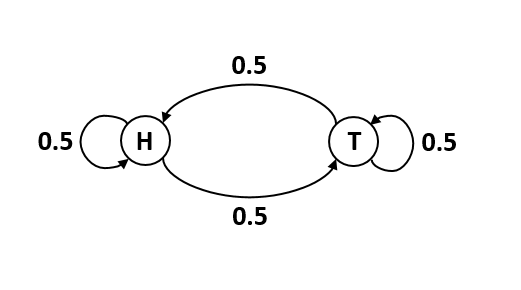
\includegraphics[scale=0.5]{MCGraph}\,.
\end{center}

A first step transition matrix $\mathbf{P}(1,0)$ is an $s\times s$ matrix, where $s = |S|$, defined by
\begin{align*}
\bmat{\mathbb{P}(s_i \to s_1)\\
\mathbb{P}(s_i \to s_2)\\
\vdots\\
\mathbb{P}(s_i \to s_s)} = \mathbf{P}(1,0)\, \vec{s}_i
\end{align*}
where $\vec{s}_i$ is the vector of the $i$-th pure state ($1$ in the $i$-th entry and $0$ elsewhere), and $s_j \in S$. Here $\mathbf{P}(1,0)$ is an example of stochastic matrix, with nonnegative entries, and each column sums up to $1$. More generally, we define $P(m+n,m)$ to be the transition matrix from $X_m$ to $X_{m+n}$. It is not hard to observe that we have
\begin{align*}
[\mathbf{P}(m+n +r, m)]_{j,i} 
&= \sum_l [\mathbf{P}(m+n+r,m+n)]_{j,l}\cdot [\mathbf{P}(m+n,m)]_{l,i} \\
&= [\mathbf{P}(m+n+r,m+n)\cdot \mathbf{P}(m+n,n)]_{j,i}\,.
\end{align*} 
If one has homogeneity in the chain, then $\mathbf{P}(m+1,m) = \mathbf{P}(1,0)$, and to conclude by induction, if the chain is homogeneous, then 
$$\mathbf{P}(k,0) = \left(\mathbf{P}(1,0)\right)^k\,,$$
or simply written as
\begin{align*}
\mathbf{P}(k) = (\mathbf{P}(1))^k\,.
\end{align*}

\section[Classification of Chains]{\color{red}Classification of Chains\color{black}}
For differential equation, one seeks for solution based on the \textit{transient}, \textit{recurrent}, and \textit{periodic} properties of the equation. In probabilistic problems, we say a a state $i$ is recurrent, or persistent, provided that we have
\begin{align*}
\mathbb{P}\left(\{X_n = i \text{ with some }n>0 | X_0 = i\}\right) = 1\,.
\end{align*}
A state $i$ is said to be transient provided that we have
\begin{align*}
\mathbb{P}\left(\{X_n = i \text{ with some }n>0 | X_0 = i\}\right) < 1\,.
\end{align*}
The recurrent state $i$ is further divided into two types, null and non-null. Let $i$ be a recurrent state, let $f_{ij}(n)$ denote the probability that the first visit to $i$ starting from $j$ in $n$ steps, and let $T_i$ be the random variable of the first return to $i$, that is
\begin{align*}
\mathbb{P}(T_i = n) = f_{ii}(n)\,.
\end{align*}
If we define
\begin{align*}
\mathbb{E}(T_i) = \sum_{n=1}^\infty n f_{ii}(n)\,,
\end{align*}
then the recurrent state is said to be null provided that $\mathbb{E}(T_i )= \infty$, and non-null provided that $\mathbb{E}(T_i) < \infty$. 

\begin{thm}[Characterization Theorem]
A state $j$ is persistent if and only if we have $\sum_n p_{jj}(n) = \infty$, and in this case, $\sum_n p_{ij}(n) = \infty$ as well whenever $f_{ij}>0$, that is some probability of transiting from $j$ to $i$. Here we denote (as they are elements of the transition matrix)
$$
p_{ij}(n) = \mathbb{P}(j \to i \text{ in $n$ steps})\,,\qquad
f_{ij}(n) = \mathbb{P}(j \to i \text{ for the first time, in $n$ steps})\,.
$$
Furthermore, $j$ is transient if and only if $
\sum_{n}p_{jj}(n) <\infty\,.$% and in such case we have $\sum_{n}p_{ij}(n) < \infty$ for all states $i$. 
\end{thm}

\example For a transition matrix $\mathbf{P}$ defined by
\begin{align*}
\mathbf{P} = \bmat{1 & 1 \\ 0 & 0}\,,
\end{align*}
we see immediately that the state $(1,0)$ is recurrent and the state $(0,1)$ is transient, and that we have also
\begin{align*}
\mathbf{P}^n =\cdots =  \mathbf{P}^2 = \mathbf{P}\,.
\end{align*}
thus we have $p_{11}(n) = 1$ and $p_{22}(n) = 0$.\\

\example On the other hand, for a transition matrix $\mathbf{P}$ defined by
\begin{align*}
\mathbf{P} = \bmat{1 & 1/2 \\ 0 & 1/2}\,,
\end{align*}
we can compute
\begin{align*}
p_{22}(n) = \frac{1}{2^n}\,,\qquad
p_{12}(n) = \frac{1}{2}+ \frac{1}{4} + \cdots + \frac{1}{2^n}\,.
\end{align*}
Thus we have
\begin{align*}
\sum_{n}p_{22}(n) <\infty\,,\qquad \sum_n p_{12}(n)=\infty\,,
\end{align*}
justifying $(0,1)$ is a transient state. 

\begin{cor}
If the phase space has dimension $|S| < \infty$, then at least one state is persistent and all states are non-null. 
\end{cor}
\begin{proof}
Here for state $j$, we have
\begin{align*}
\sum_{i=1}^{|S|} p_{ij}(n) = 1\,.
\end{align*}
Suppose that all states are transient, then we can write
\begin{align*}
1 = \lim_{n\to \infty}1 = \lim_{n\to \infty}\sum_{i=1}^{|S|}p_{ij}(n) = \sum_{i=1}^{|S|}\lim_{n\to \infty}p_{ij}(n) = \sum_{i=1}^{|S|}  0 = 0\,.
\end{align*}
Thus contradicting. The proof of non-null is left for the reader.
\end{proof}

\begin{defn}
Mean recurrence time for state $j$ can be defined by
\begin{align*}
\mu_j  = \mathbb{E}(T_j |X_0 = j) =\sum_{n}n\, f_{jj}(n) 
\end{align*}
where $T_j$ is the time for the first return back to $j$. For null persistent state $j$, one would find that we have $\mu_j = \infty$, and for non-null persistent state $i$, one would find that $\mu_i < \infty$. 
\end{defn}

\begin{defn}
The period of a state $j$ is defined to be
\begin{align*}
d(j) = \text{gcd}\{n | p_{jj}(n) > 0\}\,.
\end{align*}
If a state $i$ has $d(i) = 1$, then $i$ is a periodic. On the other hand, the state $i$ is said to be periodic  provided that $d(i) >0$. \\
\end{defn}


From here, we write $j \to i$ provided that $p_{ij}(n) >0$ for some $n$, and we say $j$ is equivalent to $i$ provided that $j\leftrightarrow i$, that is $p_{ij}(m) >0$ and $p_{ji}(n) >0$ for some $m$ and $n$. This defines an equivalence relation for states in $S$. That is, if we have $i \leftrightarrow j$ and $j\leftrightarrow k$, then $i \leftrightarrow k$. If we have $i \leftrightarrow j$, then $j \leftrightarrow i$. Given this notion, any countable space $S$ can be decomposed as $S = T \cup C_1 \cup C_2 \cup \cdots$, where $T$ is the set of transient states, and $C_i$ are closed and irreducible sets, defined by the equivalent classes of the relation $\leftrightarrow$. Note that a set $C \subseteq S$ is said to be closed provided that for $j \in C$, i $\notin C$, we have $p_{ij} = 0$. Also note that a set $C \subseteq S$ is irreducible provided that $C$ is closed and cannot be written as $C_1 \cup C_2$ with closed and disjoint sets $C_i$. 
\\

\note Suppose a class $C \subseteq S$ is closed, and $j \in C$. Then if we have $ i\leftrightarrow j$, then $i \in C$, as we have $p_{ij}(n) > 0$, which is impossible if $i$ is outside of $C$. Furthermore, if the class is not closed, then we must have
\begin{align*}
\mathbb{P}\left(\{X_n = j\} \cap \{X_r = i\text{ for infinitely many times}\} |X_0 = i\right) = 0
\end{align*}
for $i \in C$ and $j \notin C$. Here we denote
\begin{align*}
\mathbb{P}_i(A) = \mathbb{P}(A |X_0=i) 
\end{align*}
for any condition $A$.\\

\note For a class $C \subseteq S$, if $i \in C$ is transient, then all $j \in C$ are transient. That is, if $i \in C$ is transient, then
\begin{align*}
\sum_n p_{ii}(n) < \infty\,,
\end{align*}
and for $j \in C$, $j \leftrightarrow i$, and thus $p_{ij}(n) > 0$, $p_{ji}(n) > 0$, so we can write, for any $r \geq 1$, 
\begin{align*}
p_{ji}(m+n+r) \geq p_{ji}(m)\, p_{ii}(r) \, p_{ij}(n)\,.
\end{align*}
Then we see that
\begin{align*}
\infty> \sum_{k=1}^\infty p_{ii}(k) \geq \sum_r p_{ii}(m+n+r) \geq \sum_{r=1}^\infty p_{ij}(m)\, p_{jj}(r) \, p_{ji}(n) = p_{ij}(m)\, p_{ji}(n) \, \sum_{r=1}^\infty p_{jj}(r)\,,
\end{align*}
the desired result thus follows. 

\example For simple random walk, we have $S = \Z$ and $\Z$ is closed and irreducible. \\

Now consider we are given a transition matrix $\mathbf{P}$, and we denote a state $\pi = (\cdots, \pi_i , \cdots)$ with $\pi_i \geq 0$ for all $i$ and $\sum_{i}\pi_i = 1$. Then
\begin{align*}
\mathbf{P}\pi = \pi
\end{align*} 
is in fact an eigenvalue problem, but with extra condition that $\pi_i \geq 0$ for all $i$ and $\sum_i \pi_i < \infty$. For finite state system, with $|S| = s < \infty$, we have the Perron-Frobenius Theorem.
\begin{thm}[Perron-Frobenius Theorem]
Let $\mathbb{P}$ be the transition matrix of a finite irreducible chain $S$ with period $d$, then $\lambda = 1$ is an eigenvalue of $\mathbb{P}$ with multiplicity $1$. The other eigenvalues of $\mathbf{P}$, denoted as $\lambda_i$ with $2\leq i \leq s$, satisfies $|\lambda_i | < 1$. Furthermore, there exists a unique $\pi \in \R^s$ such that $\pi_i \geq 0$, and $\sum_i \pi_i = 1$. 
\end{thm}

An $n\times n$ stochastic matrix is said to have boredom terms if it consists of all terms to be $1/n$. Note that for an arbitrary stochastic $n\times n$ matrix $P$ and a boredom matrix $B$, $(1-t)P + tB$ is also a stochastic matrix when $t \in [0,1]$. 

\end{document}


